\documentclass[11pt,a4paper]{article}

% ── Packages ──
\usepackage[utf8]{inputenc}
\usepackage[T1]{fontenc}
% \usepackage{lmodern}
\usepackage[margin=2.4cm]{geometry}
\usepackage{amsmath,amssymb,amsthm,mathtools}
\usepackage{braket}
\usepackage{physics}
% \usepackage{bbm}  % not available
\usepackage{tikz}
\usetikzlibrary{arrows.meta,positioning,calc,decorations.pathmorphing,patterns,shapes.geometric,fit,backgrounds}
\usepackage{pgfplots}
\pgfplotsset{compat=1.16}
\usepackage{hyperref}
\usepackage{cleveref}
\usepackage{enumitem}
\usepackage{booktabs}
\usepackage{array}
\usepackage{caption}

% ── Theorem environments ──
\newtheorem{theorem}{Theorem}[section]
\newtheorem{proposition}[theorem]{Proposition}
\newtheorem{lemma}[theorem]{Lemma}
\newtheorem{corollary}[theorem]{Corollary}
\theoremstyle{definition}
\newtheorem{definition}[theorem]{Definition}
\newtheorem{example}[theorem]{Example}
\theoremstyle{remark}
\newtheorem{remark}[theorem]{Remark}

% ── Custom commands ──
\newcommand{\HH}{\mathcal{H}}
\newcommand{\PP}{\mathcal{P}}
\newcommand{\Mlin}{M_{\mathrm{lin}}}
\newcommand{\Mtwo}{\overline{M}_2}
\newcommand{\UFT}{U^{\mathrm{FT}}}
\newcommand{\AQFT}{\mathrm{AQFT}}
\newcommand{\MPO}{\mathrm{MPO}}
\newcommand{\MPS}{\mathrm{MPS}}
\newcommand{\QFT}{\mathrm{QFT}}
\newcommand{\DFT}{\mathrm{DFT}}
\newcommand{\id}{\mathbf{1}}
\renewcommand{\Tr}{\mathrm{Tr}}
\newcommand{\ee}{\mathrm{e}}
\newcommand{\ii}{\mathrm{i}}
%\DeclareMathOperator{\rank}{rank}

% ══════════════════════════════════════════════════════════════
\begin{document}

\title{\textbf{Non-Stabilizing Power of the Quantum Fourier Transform\\[4pt]
via Matrix Product Operator Representation}}
\author{Working Notes}
\date{\today}
\maketitle

\begin{abstract}
We develop an analytical framework for computing the non-stabilizing power (magic power) of the quantum Fourier transform (QFT) using its matrix product operator (MPO) representation.
The recently established interpolative MPO construction of Chen \& Lindsey provides a closed-form, translationally invariant tensor network for the QFT with bond dimension $r=K+1$.
We exploit this structure to reformulate the computation of the linear magic power $\Mlin(\UFT)$ as a transfer-matrix problem on the four-replica Hilbert space.
Starting from the single-qubit case (Hadamard gate) and building through two and three qubits, we derive the general transfer-matrix formalism and analyse the thermodynamic limit $n\to\infty$.
In this limit, the magic power per site is governed by the leading eigenvalue of a $(K+1)^8$-dimensional transfer matrix, and we show that it converges to a well-defined intensive quantity.
\end{abstract}

\tableofcontents
\newpage

% ══════════════════════════════════════════════════════════════
\section{Introduction}
\label{sec:intro}

The quantum Fourier transform (QFT) is a cornerstone of quantum computation.
Beyond its algorithmic significance, the QFT provides a rich setting for studying non-stabilizerness (``magic''), a resource that quantifies the deviation of quantum states and operations from the efficiently simulable stabilizer formalism.

The non-stabilizing power of a unitary $U$ quantifies how much magic it can generate when applied to stabilizer states, averaged over the Clifford group:
\begin{equation}\label{eq:magic_power_def}
  \Mlin(U) = \mathbb{E}_{C}[\Mlin(UC\ket{0}^{\otimes n})]\,,
\end{equation}
where $\Mlin(\ket{\psi}) = 1 - d\,\Tr[Q\,\psi^{\otimes 4}]$ is the linear stabilizer R\'enyi entropy, $d=2^n$, and $Q = d^{-2}\sum_{P\in\PP_n} P^{\otimes 4}$ is the projector onto the Pauli-symmetric subspace of four replicas.

Computing $\Mlin(\UFT)$ directly requires manipulating objects of dimension $d^4 = 2^{4n}$, which is intractable for large $n$.
The key insight of this work is to exploit the MPO representation of $\UFT$ established by Chen and Lindsey~\cite{ChenLindsey2026}, which compresses the $2^n\times 2^n$ DFT matrix into a tensor network with bond dimension $r = K+1$ and \emph{translationally invariant} cores.
Combined with the local structure of the projector $Q$ and the permutation operators $T_\pi$ in the replica space, this reduces the computation of $\Mlin(\UFT)$ to a \emph{transfer-matrix contraction} that scales polynomially in $r$ and linearly in $n$.

The outline is as follows.
In \cref{sec:mpo} we review the MPO construction of the QFT.
In \cref{sec:magic_review} we recall the formula for the non-stabilizing power.
In \cref{sec:warmup} we work out the cases $n=1,2$ explicitly.
In \cref{sec:transfer} we develop the general transfer-matrix formalism.
In \cref{sec:thermo} we analyse the thermodynamic limit.
In \cref{sec:aqft} we compare with the approximate QFT.

\begin{figure}[ht]
\centering
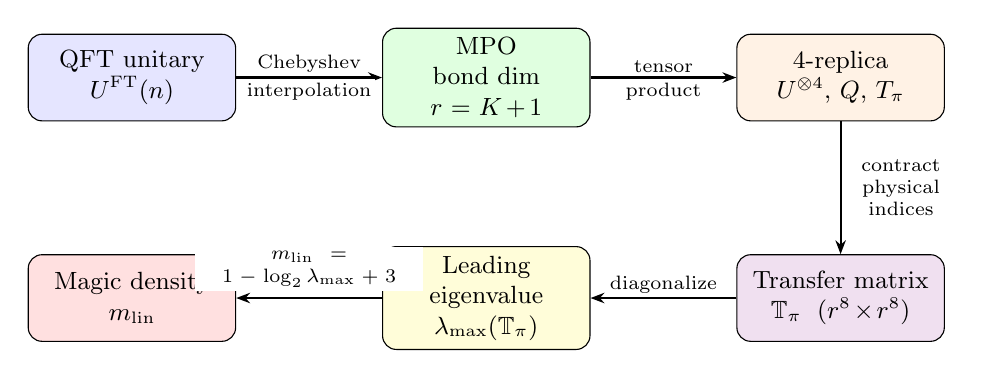
\begin{tikzpicture}[
    box/.style={draw, rounded corners=5pt, fill=#1, minimum width=2.6cm, minimum height=1.1cm, text width=2.4cm, align=center, font=\small},
    box/.default={gray!8},
    arr/.style={-{Stealth[length=5pt]}, thick},
    lbl/.style={font=\scriptsize, fill=white, inner sep=1.5pt},
]
% Top row: left to right
\node[box=blue!10] (qft) at (0,0) {QFT unitary\\$\UFT(n)$};
\node[box=green!12] (mpo) at (4.5,0) {MPO\\bond dim $r\!=\!K\!+\!1$};
\node[box=orange!10] (rep) at (9.0,0) {4-replica\\$U^{\otimes 4}$, $Q$, $T_\pi$};

% Bottom row: right to left
\node[box=violet!12] (tm)  at (9.0,-2.8) {Transfer matrix\\$\mathbb{T}_\pi$\; $(r^8\!\times\! r^8)$};
\node[box=yellow!15] (eig) at (4.5,-2.8) {Leading eigenvalue\\$\lambda_{\max}(\mathbb{T}_\pi)$};
\node[box=red!12] (mag)    at (0,-2.8) {Magic density\\$m_{\mathrm{lin}}$};

% Arrows: top row
\draw[arr] (qft) -- node[lbl, above] {Chebyshev} node[lbl, below] {interpolation} (mpo);
\draw[arr] (mpo) -- node[lbl, above] {tensor} node[lbl, below] {product} (rep);

% Arrow: down
\draw[arr] (rep) -- node[lbl, right, text width=1.4cm, align=center] {contract\\physical\\indices} (tm);

% Arrows: bottom row (right to left)
\draw[arr] (tm) -- node[lbl, above] {diagonalize} (eig);
\draw[arr] (eig) -- node[lbl, above=2pt, text width=2.8cm, align=center] {$m_{\mathrm{lin}} = 1 - \log_2\lambda_{\max} + 3$} (mag);

\end{tikzpicture}
\caption{Conceptual overview of the approach.
The QFT is compressed into an MPO via Chebyshev interpolation; the magic power formula involves traces over four replicas that factorize into a transfer-matrix chain; the thermodynamic magic density is governed by the leading eigenvalue.}
\label{fig:overview}
\end{figure}

% ══════════════════════════════════════════════════════════════
\section{MPO Representation of the QFT}
\label{sec:mpo}

\subsection{Quantized tensor representation}

The DFT matrix of size $N=2^n$ has entries
\begin{equation}\label{eq:DFT}
  \mathbf{F}_{s,t} = \ee^{-2\pi\ii\, st/N}\,.
\end{equation}
We introduce qubit indices $\sigma_k, \tau_k \in \{0,1\}$ via
\begin{equation}\label{eq:binary}
  s = \sum_{k=1}^n 2^{n-k}\sigma_k\,, \qquad
  t = \sum_{l=1}^n 2^{l-1}\tau_l\,,
\end{equation}
with \emph{opposite} bit orderings for $s$ and $t$. Then
\begin{equation}\label{eq:F_tensor}
  F(\sigma_{1:n},\tau_{1:n}) = \ee^{-\pi\ii \sum_{k,l=1}^n 2^{-k}2^l \sigma_k\tau_l}\,.
\end{equation}
We seek an MPO approximation:
\begin{equation}\label{eq:MPO_def}
  F(\sigma_{1:n},\tau_{1:n}) \approx \sum_{\alpha_1,\ldots,\alpha_{n-1}}
  A_1^{\alpha_1}(\sigma_1,\tau_1)\,
  A^{\alpha_1\alpha_2}(\sigma_2,\tau_2)\,\cdots\,
  A^{\alpha_{n-2}\alpha_{n-1}}(\sigma_{n-1},\tau_{n-1})\,
  A_n^{\alpha_{n-1}}(\sigma_n,\tau_n)\,,
\end{equation}
where each $\alpha_k$ runs over $\{0,\ldots,K\}$ and $K+1$ is the bond dimension.

\begin{figure}[ht]
\centering
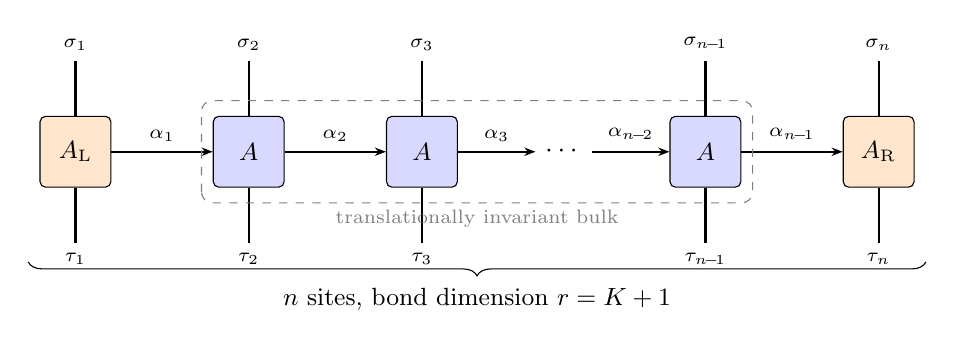
\begin{tikzpicture}[
    core/.style={draw, fill=blue!15, minimum width=0.9cm, minimum height=0.9cm, rounded corners=2pt, font=\small},
    bcore/.style={draw, fill=orange!20, minimum width=0.9cm, minimum height=0.9cm, rounded corners=2pt, font=\small},
    bond/.style={thick, -{Stealth[length=4pt]}},
    phys/.style={thick},
    lbl/.style={font=\scriptsize, midway},
]
% Left boundary
\node[bcore] (A1) at (0,0) {$A_{\mathrm{L}}$};
% Internal cores
\node[core] (A2) at (2.2,0) {$A$};
\node[core] (A3) at (4.4,0) {$A$};
\node (dots) at (6.2,0) {$\cdots$};
\node[core] (A4) at (8.0,0) {$A$};
% Right boundary
\node[bcore] (A5) at (10.2,0) {$A_{\mathrm{R}}$};

% Bond indices (horizontal lines)
\draw[bond] (A1.east) -- node[above, lbl] {$\alpha_1$} (A2.west);
\draw[bond] (A2.east) -- node[above, lbl] {$\alpha_2$} (A3.west);
\draw[bond] (A3.east) -- node[above, lbl] {$\alpha_3$} (dots.west);
\draw[bond] (dots.east) -- node[above, lbl] {$\alpha_{n\!-\!2}$} (A4.west);
\draw[bond] (A4.east) -- node[above, lbl] {$\alpha_{n\!-\!1}$} (A5.west);

% Physical legs (up = sigma, down = tau)
\foreach \nd/\lab in {A1/1, A2/2, A3/3, A4/{n\!-\!1}, A5/n} {
  \draw[phys] (\nd.north) -- ++(0,0.7) node[above, font=\scriptsize] {$\sigma_{\lab}$};
  \draw[phys] (\nd.south) -- ++(0,-0.7) node[below, font=\scriptsize] {$\tau_{\lab}$};
}

% Annotations
\draw[decorate, decoration={brace, amplitude=5pt, mirror}] (-0.6,-1.4) -- (10.8,-1.4)
  node[midway, below=6pt, font=\small] {$n$ sites, bond dimension $r=K+1$};

% Highlight translational invariance
\draw[dashed, gray, rounded corners=4pt] (1.6,-0.65) rectangle (8.6,0.65);
\node[gray, font=\scriptsize] at (5.1, -0.85) {translationally invariant bulk};
\end{tikzpicture}
\caption{Tensor network diagram of the QFT as a matrix product operator (MPO).
Each box represents a tensor core with physical indices $\sigma_k$ (output, top) and $\tau_k$ (input, bottom), connected by bond indices $\alpha_k$ of dimension $r=K+1$.
The internal cores (blue, dashed box) are all \emph{identical}, while the boundary cores (orange) differ.}
\label{fig:mpo_structure}
\end{figure}

\subsection{The key factorization}

Splitting the exponent in \eqref{eq:F_tensor} at site $m$, the cross-terms with $k\le m$, $l>m$ contribute only even integers in the exponent, hence:
\begin{equation}\label{eq:factorization}
  F(\sigma_{1:n},\tau_{1:n}) = F(\sigma_{1:m},\tau_{1:m})\;
  F(\sigma_{m+1:n},\tau_{m+1:n})\;
  \ee^{-2\pi\ii\, x_{>m}\, y_{\le m}}\,,
\end{equation}
where we defined the ``fractional-bit'' variables
\begin{equation}\label{eq:xy_def}
  x_{>m} = \sum_{k=m+1}^n 2^{m-k}\sigma_k \in [0,1]\,,\qquad
  y_{\le m} = \sum_{l=1}^m 2^{l-m-1}\tau_l \in [0,1]\,.
\end{equation}
The left--right coupling is entirely captured by the function $f_y(x) = \ee^{-2\pi\ii xy}$ for $x,y\in[0,1]$.

\begin{figure}[ht]
\centering
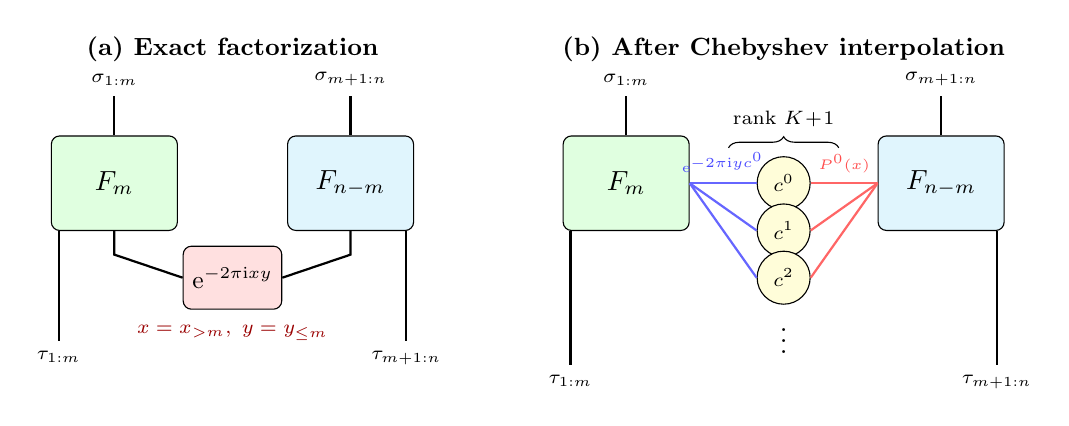
\begin{tikzpicture}[
    block/.style={draw, fill=#1, minimum width=1.6cm, minimum height=1.2cm, rounded corners=3pt},
    block/.default={green!12},
    coupling/.style={draw, fill=red!12, minimum width=1.2cm, minimum height=0.8cm, rounded corners=3pt, font=\small},
    interp/.style={draw, fill=yellow!15, circle, minimum size=0.5cm, font=\scriptsize},
    >=Stealth,
]
% === Left panel: exact factorization ===
\node[font=\small\bfseries] at (0, 2.3) {(a) Exact factorization};

\node[block=green!12] (FL) at (-1.5,0.6) {$F_m$};
\node[block=cyan!12] (FR) at (1.5,0.6) {$F_{n-m}$};
\node[coupling] (coup) at (0,-0.6) {$\ee^{-2\pi\ii x y}$};

% Physical legs
\draw[thick] (FL.north) -- ++(0,0.5) node[above,font=\scriptsize] {$\sigma_{1:m}$};
\draw[thick] (FL.south) -- ++(0,-0.3) -- (coup.west);
\draw[thick] (FR.north) -- ++(0,0.5) node[above,font=\scriptsize] {$\sigma_{m+1:n}$};
\draw[thick] (FR.south) -- ++(0,-0.3) -- (coup.east);
\draw[thick] (FL.south west) ++(0.1,0) -- ++(0,-1.4) node[below,font=\scriptsize] {$\tau_{1:m}$};
\draw[thick] (FR.south east) ++(-0.1,0) -- ++(0,-1.4) node[below,font=\scriptsize] {$\tau_{m+1:n}$};

% Labels
\node[font=\scriptsize, red!60!black] at (0,-1.3) {$x=x_{>m},\; y=y_{\le m}$};

% === Right panel: after interpolation ===
\node[font=\small\bfseries] at (7, 2.3) {(b) After Chebyshev interpolation};

\node[block=green!12] (FL2) at (5.0,0.6) {$F_m$};
\node[block=cyan!12] (FR2) at (9.0,0.6) {$F_{n-m}$};

% Interpolation nodes
\foreach \i/\a in {0/0, 1/1, 2/2} {
  \node[interp] (c\i) at (7, 0.6-0.6*\i) {$c^{\a}$};
}
\node at (7, -1.3) {$\vdots$};

% Connections
\draw[thick, blue!60] (FL2.east) -- (c0.west) node[above, midway, font=\tiny, blue!70] {$\ee^{-2\pi\ii y c^0}$};
\draw[thick, blue!60] (FL2.east) -- (c1.west);
\draw[thick, blue!60] (FL2.east) -- (c2.west);

\draw[thick, red!60] (c0.east) -- (FR2.west) node[above, midway, font=\tiny, red!70] {$P^0(x)$};
\draw[thick, red!60] (c1.east) -- (FR2.west);
\draw[thick, red!60] (c2.east) -- (FR2.west);

% Physical legs
\draw[thick] (FL2.north) -- ++(0,0.5) node[above,font=\scriptsize] {$\sigma_{1:m}$};
\draw[thick] (FL2.south west) ++(0.1,0) -- ++(0,-1.7) node[below,font=\scriptsize] {$\tau_{1:m}$};
\draw[thick] (FR2.north) -- ++(0,0.5) node[above,font=\scriptsize] {$\sigma_{m+1:n}$};
\draw[thick] (FR2.south east) ++(-0.1,0) -- ++(0,-1.7) node[below,font=\scriptsize] {$\tau_{m+1:n}$};

% Bond label
\draw[decorate, decoration={brace, amplitude=4pt}] (6.3,1.05) -- (7.7,1.05)
  node[midway, above=4pt, font=\scriptsize] {rank $K\!+\!1$};

\end{tikzpicture}
\caption{(a)~The DFT tensor factorizes into left and right blocks coupled by the phase $\ee^{-2\pi\ii xy}$.
(b)~Chebyshev--Lobatto interpolation of the coupling function inserts a rank-$(K\!+\!1)$ decomposition through the interpolation nodes $c^\alpha$.  The left factor contributes $\ee^{-2\pi\ii y\,c^\alpha}$ and the right contributes $P^\alpha(x)$.}
\label{fig:factorization}
\end{figure}

\subsection{Chebyshev--Lobatto interpolation and the tensor core}

We approximate $f_y(x)$ using $(K+1)$-point Chebyshev--Lobatto interpolation. The nodes are
\begin{equation}\label{eq:cheb_nodes}
  c^\alpha = \frac{1-\cos(\pi\alpha/K)}{2}\,,\qquad \alpha=0,\ldots,K\,,
\end{equation}
and the Lagrange interpolating polynomials satisfy $P^\alpha(c^\beta) = \delta_{\alpha\beta}$ and $\sum_\alpha P^\alpha(x)=1$.

The recursion $y_{\le m+1} = \tfrac{1}{2}y_{\le m} + \tfrac{1}{2}\tau_{m+1}$ leads to the interpolative decomposition
\begin{equation}
  f_{y_{\le m}}\!\Bigl(\frac{\sigma_{m+1}+c^\beta}{2}\Bigr)
  \approx \sum_{\alpha=0}^K \ee^{-2\pi\ii\, y_{\le m}\, c^\alpha}\;
  P^\alpha\!\Bigl(\frac{\sigma_{m+1}+c^\beta}{2}\Bigr)\,,
\end{equation}
from which one obtains the \textbf{translationally invariant tensor core}:
\begin{equation}\label{eq:core}
  \boxed{
  A^{\alpha\beta}(\sigma,\tau) = P^\alpha\!\Bigl(\frac{\sigma+c^\beta}{2}\Bigr)\;
  \ee^{-\pi\ii(\sigma+c^\beta)\tau}\,,\qquad
  \sigma,\tau\in\{0,1\},\quad \alpha,\beta\in\{0,\ldots,K\}\,.
  }
\end{equation}
The boundary conditions are:
\begin{align}
  A_{\mathrm{L}}^\beta(\sigma,\tau) &= \ee^{-\pi\ii(\sigma+c^\beta)\tau}
  \qquad\text{(leftmost core)}\,,\label{eq:left_core}\\
  A_{\mathrm{R}}^\alpha(\sigma,\tau) &= P^\alpha(\sigma/2)\;\ee^{-\pi\ii\sigma\tau}
  \qquad\text{(rightmost core)}\,.\label{eq:right_core}
\end{align}

\subsection{Error bounds}

The entrywise error of the MPO satisfies (Theorem~4 of~\cite{ChenLindsey2026}):
\begin{equation}\label{eq:error_bound}
  \|F_{\MPO} - F\|_\infty \le (n-1)\,\Lambda_K^{n-2}\, E_K\,,
\end{equation}
where $\Lambda_K \le 1+\frac{2}{\pi}\log(K+1)$ is the Lebesgue constant and
\begin{equation}
  E_K \le \frac{4\bigl(\frac{\pi}{2}\bigr)^{K+1}\ee^K\, K^{-K}}{K-\frac{\pi}{2}}
\end{equation}
decays super-exponentially with $K$.  For instance, $K=6$ yields $E_6 \approx 2.6\times 10^{-4}$, and $K=10$ gives $E_{10}\approx 5.3\times10^{-9}$.

% ══════════════════════════════════════════════════════════════
\section{Magic Power: General Formula}
\label{sec:magic_review}

\subsection{Definitions}

For an $n$-qubit system with $d=2^n$, the $n$-qubit Pauli group (modulo phases) is $\PP_n$, and the key operators on $\HH^{\otimes 4}$ are:
\begin{align}
  Q &= \frac{1}{d^2}\sum_{P\in\PP_n} P^{\otimes 4}\,,\label{eq:Q}\\
  \Pi_{\mathrm{sym}} &= \frac{1}{4!}\sum_{\pi\in S_4} T_\pi\,,\label{eq:Pisym}
\end{align}
where $T_\pi$ permutes the four replicas according to $\pi\in S_4$.

The linear non-stabilizing power of a unitary $U$ is
\begin{equation}\label{eq:Mlin_general}
  \boxed{
  \Mlin(U) = \frac{d}{d+4} -
  \frac{d\bigl[3\,\Tr(QU^{\dagger\otimes 4}QU^{\otimes 4}T_{(34)})
    + \Tr(QU^{\dagger\otimes 4}QU^{\otimes 4})
    + 2\,\Tr(QU^{\dagger\otimes 4}QU^{\otimes 4}T_{(123)})\bigr]}
       {(d+1)(d+2)(d+4)}
  }
\end{equation}

The three traces in the numerator --- which we call $\mathcal{T}_{\mathrm{id}}$, $\mathcal{T}_{(34)}$, $\mathcal{T}_{(123)}$ --- constitute the main computational challenge.

\subsection{Structure of the traces}

All three have the form
\begin{equation}\label{eq:trace_general}
  \mathcal{T}_\pi = \Tr\bigl(Q\,U^{\dagger\otimes 4}\,Q\,U^{\otimes 4}\,T_\pi\bigr)\,,
\end{equation}
where $T_\pi$ is the identity for $\mathcal{T}_{\mathrm{id}}$, the swap $(34)$ for $\mathcal{T}_{(34)}$, and the 3-cycle $(123)$ for $\mathcal{T}_{(123)}$.

The crucial observation is that each of $Q$, $T_\pi$, and $U^{\otimes 4}$ (when $U$ is an MPO) factorizes over the $n$ qubit sites, enabling the trace to be computed as a \emph{transfer-matrix product}.

\begin{figure}[ht]
\centering
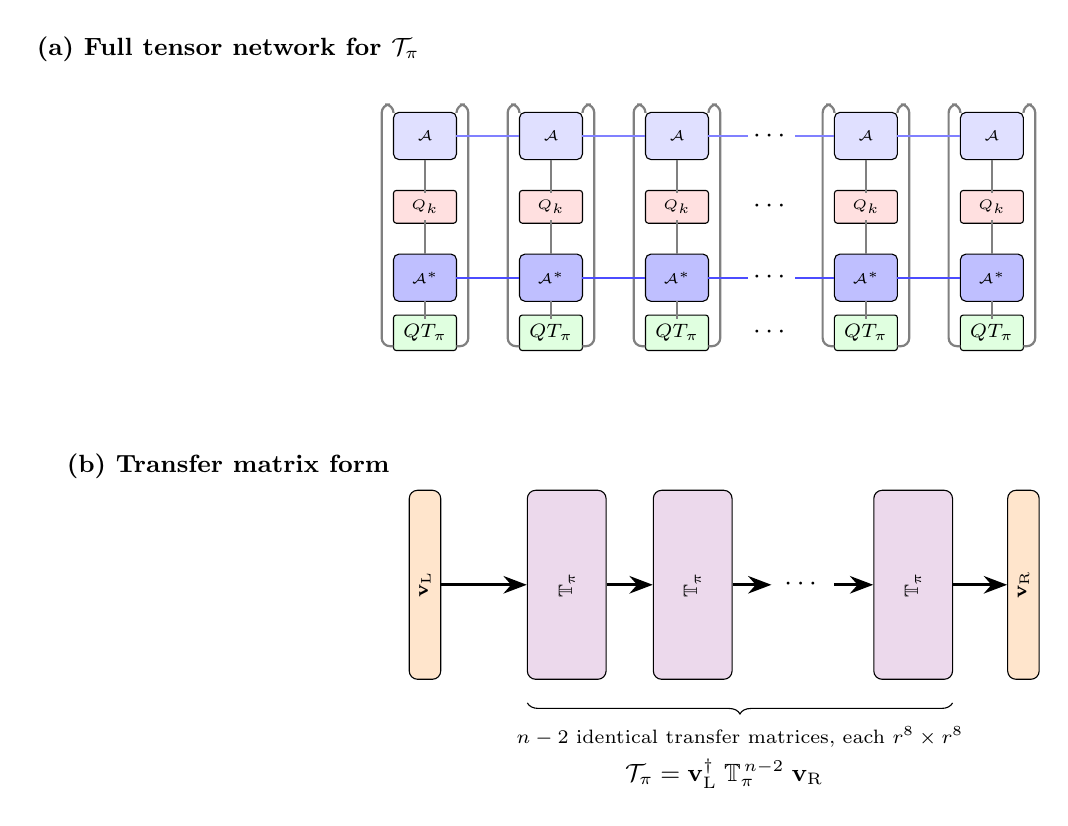
\begin{tikzpicture}[
    core/.style={draw, fill=blue!12, minimum width=0.8cm, minimum height=0.6cm, rounded corners=2pt, font=\tiny},
    corec/.style={draw, fill=blue!25, minimum width=0.8cm, minimum height=0.6cm, rounded corners=2pt, font=\tiny},
    qbox/.style={draw, fill=red!12, minimum width=0.8cm, minimum height=0.35cm, rounded corners=1pt, font=\tiny},
    tbox/.style={draw, fill=green!12, minimum width=0.8cm, minimum height=0.35cm, rounded corners=1pt, font=\tiny},
    tm/.style={draw, fill=violet!15, minimum width=1.0cm, minimum height=2.4cm, rounded corners=3pt, font=\scriptsize},
    bvec/.style={draw, fill=orange!20, minimum width=0.4cm, minimum height=2.4cm, rounded corners=3pt, font=\scriptsize},
    >=Stealth,
]
% === Top panel: full tensor network ===
\node[font=\small\bfseries] at (-2.5, 3.3) {(a) Full tensor network for $\mathcal{T}_\pi$};

\foreach \x/\idx in {0/1, 1.6/2, 3.2/3, 5.6/4, 7.2/5} {
  % U^{otimes 4}
  \node[core] (U\idx) at (\x, 2.2) {$\mathcal{A}$};
  % U^{dag otimes 4}
  \node[corec] (Ud\idx) at (\x, 0.4) {$\mathcal{A}^*$};
  % Q on top
  \node[qbox] (Qt\idx) at (\x, 1.3) {$Q_k$};
  % Q T_pi on bottom (connecting)
}
% T_pi at bottom
\node[tbox] at (0, -0.3) {\scriptsize$Q T_\pi$};
\node[tbox] at (1.6, -0.3) {\scriptsize$Q T_\pi$};
\node[tbox] at (3.2, -0.3) {\scriptsize$Q T_\pi$};
\node[tbox] at (5.6, -0.3) {\scriptsize$Q T_\pi$};
\node[tbox] at (7.2, -0.3) {\scriptsize$Q T_\pi$};

% dots
\node at (4.4, 2.2) {$\cdots$};
\node at (4.4, 0.4) {$\cdots$};
\node at (4.4, 1.3) {$\cdots$};
\node at (4.4, -0.3) {$\cdots$};

% Vertical connections (physical indices traced)
\foreach \x in {0, 1.6, 3.2, 5.6, 7.2} {
  \draw[thick, gray] (\x, 2.2-0.3) -- (\x, 1.3+0.17);
  \draw[thick, gray] (\x, 1.3-0.17) -- (\x, 0.4+0.3);
  \draw[thick, gray] (\x, 0.4-0.3) -- (\x, -0.3+0.17);
  % Loop from bottom back to top (trace)
  \draw[thick, gray, rounded corners=3pt] (\x+0.4, -0.3-0.17) -- (\x+0.55, -0.3-0.17) -- (\x+0.55, 2.6) -- (\x+0.4, 2.6) -- (\x+0.4, 2.2+0.3);
  \draw[thick, gray, rounded corners=3pt] (\x-0.4, -0.3-0.17) -- (\x-0.55, -0.3-0.17) -- (\x-0.55, 2.6) -- (\x-0.4, 2.6) -- (\x-0.4, 2.2+0.3);
}
% Horizontal bonds
\foreach \xa/\xb in {0/1.6, 1.6/3.2, 5.6/7.2} {
  \draw[thick, blue!50] (\xa+0.4, 2.2) -- (\xb-0.4, 2.2);
  \draw[thick, blue!70] (\xa+0.4, 0.4) -- (\xb-0.4, 0.4);
}
\draw[thick, blue!50] (3.2+0.4, 2.2) -- (4.1, 2.2);
\draw[thick, blue!50] (4.7, 2.2) -- (5.6-0.4, 2.2);
\draw[thick, blue!70] (3.2+0.4, 0.4) -- (4.1, 0.4);
\draw[thick, blue!70] (4.7, 0.4) -- (5.6-0.4, 0.4);

% === Bottom panel: transfer matrix chain ===
\node[font=\small\bfseries] at (-2.5, -2.0) {(b) Transfer matrix form};

\node[bvec] (vL) at (0, -3.5) {\rotatebox{90}{$\mathbf{v}_{\mathrm{L}}$}};
\node[tm] (T1) at (1.8, -3.5) {\rotatebox{90}{$\mathbb{T}_\pi$}};
\node[tm] (T2) at (3.4, -3.5) {\rotatebox{90}{$\mathbb{T}_\pi$}};
\node at (4.8, -3.5) {$\cdots$};
\node[tm] (T3) at (6.2, -3.5) {\rotatebox{90}{$\mathbb{T}_\pi$}};
\node[bvec] (vR) at (7.6, -3.5) {\rotatebox{90}{$\mathbf{v}_{\mathrm{R}}$}};

\draw[very thick, -{Stealth}] (vL.east) -- (T1.west);
\draw[very thick, -{Stealth}] (T1.east) -- (T2.west);
\draw[very thick, -{Stealth}] (T2.east) -- (4.4, -3.5);
\draw[very thick, -{Stealth}] (5.2, -3.5) -- (T3.west);
\draw[very thick, -{Stealth}] (T3.east) -- (vR.west);

% Dimension labels
\draw[decorate, decoration={brace, amplitude=4pt, mirror}] (1.3,-5.0) -- (6.7,-5.0)
  node[midway, below=5pt, font=\scriptsize] {$n-2$ identical transfer matrices, each $r^8\times r^8$};

% Result
\node[font=\small] at (3.8, -5.9) {$\mathcal{T}_\pi = \mathbf{v}_{\mathrm{L}}^\dagger\;\mathbb{T}_\pi^{\,n-2}\;\mathbf{v}_{\mathrm{R}}$};
\end{tikzpicture}
\caption{(a)~The trace $\mathcal{T}_\pi = \Tr(Q\,U^{\dagger\otimes 4}\,Q\,U^{\otimes 4}\,T_\pi)$ as a two-dimensional tensor network.
Each column corresponds to one qubit site; vertical lines are physical indices (traced over), horizontal lines are bond indices.
(b)~Contracting each column yields a transfer matrix $\mathbb{T}_\pi$, reducing the computation to a matrix product.
The boundary vectors $\mathbf{v}_{\mathrm{L}}, \mathbf{v}_{\mathrm{R}}$ encode the boundary MPO cores.}
\label{fig:transfer_matrix}
\end{figure}

% ══════════════════════════════════════════════════════════════
\section{Warm-Up: Small Systems}
\label{sec:warmup}

\subsection{One qubit: the Hadamard gate}

For $n=1$, the QFT reduces to the Hadamard gate $H = (X+Z)/\sqrt{2}$, which is a Clifford unitary. Since Clifford unitaries map Pauli operators to Pauli operators, $[H^{\otimes 4}, Q\Pi_{\mathrm{sym}}]=0$, and therefore
\begin{equation}
  \Mlin(H) = 0\,.
\end{equation}
This is consistent with the general result $\Mlin(C)=0$ for any Clifford $C$.

\textbf{Verification via the MPO.} For $n=1$, the MPO consists of a single core $A_1$, with no bond indices. We have $A_1(\sigma,\tau) = \ee^{-\pi\ii\sigma\tau}$, which is simply $\text{diag}(1, 1, 1, -1)$ when written as a $2\times2$ matrix --- this is the Hadamard gate (in a different basis convention). The trace $\mathcal{T}_{\mathrm{id}} = \Tr(Q H^{\dagger\otimes 4} Q H^{\otimes 4})$ can be computed directly:
\begin{equation}
  \Tr(Q\,H^{\dagger\otimes 4}\,Q\,H^{\otimes 4}) = 4\,,
\end{equation}
which, combined with the analogous traces $\mathcal{T}_{(34)} = 4$ and $\mathcal{T}_{(123)}=4$, gives $\Mlin = 0$ from \eqref{eq:Mlin_general} with $d=2$.

\subsection{Two qubits: emergence of magic}
\label{sec:two_qubits}

\begin{figure}[ht]
\centering
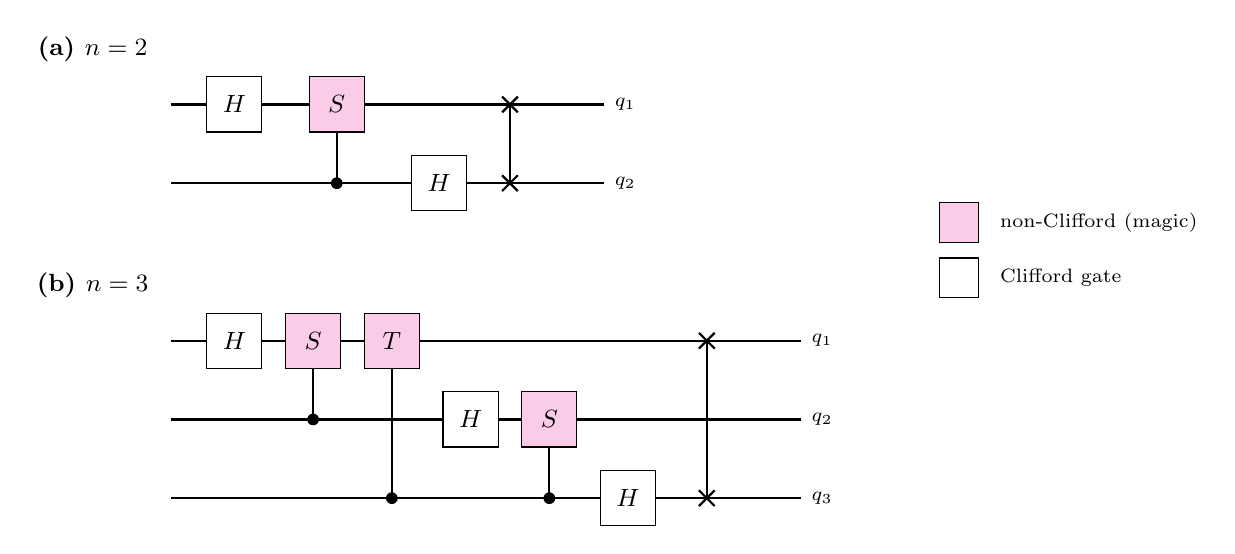
\begin{tikzpicture}[
    gate/.style={draw, fill=white, minimum width=0.7cm, minimum height=0.7cm, font=\small},
    mgate/.style={draw, fill=magenta!20, minimum width=0.7cm, minimum height=0.7cm, font=\small},
    ctrl/.style={fill=black, circle, inner sep=1.5pt},
    wire/.style={thick},
    >=Stealth,
]
% === n=2 circuit ===
\node[font=\small\bfseries] at (-1.5, 1.2) {(a) $n=2$};
\draw[wire] (-0.5,0.5) -- (5.0,0.5) node[right, font=\scriptsize] {$q_1$};
\draw[wire] (-0.5,-0.5) -- (5.0,-0.5) node[right, font=\scriptsize] {$q_2$};

\node[gate] at (0.3,0.5) {$H$};
\node[mgate] at (1.6,0.5) {$S$};
\node[ctrl] at (1.6,-0.5) {};
\draw[thick] (1.6,-0.5) -- (1.6,0.15);
\node[gate] at (2.9,-0.5) {$H$};
% SWAP
\draw[thick] (3.8,0.5) -- (3.8,-0.5);
\draw[thick] (3.8-0.1,0.5+0.1) -- (3.8+0.1,0.5-0.1);
\draw[thick] (3.8-0.1,0.5-0.1) -- (3.8+0.1,0.5+0.1);
\draw[thick] (3.8-0.1,-0.5+0.1) -- (3.8+0.1,-0.5-0.1);
\draw[thick] (3.8-0.1,-0.5-0.1) -- (3.8+0.1,-0.5+0.1);

% === n=3 circuit ===
\node[font=\small\bfseries] at (-1.5, -1.8) {(b) $n=3$};
\draw[wire] (-0.5,-2.5) -- (7.5,-2.5) node[right, font=\scriptsize] {$q_1$};
\draw[wire] (-0.5,-3.5) -- (7.5,-3.5) node[right, font=\scriptsize] {$q_2$};
\draw[wire] (-0.5,-4.5) -- (7.5,-4.5) node[right, font=\scriptsize] {$q_3$};

\node[gate] at (0.3,-2.5) {$H$};
\node[mgate] at (1.3,-2.5) {$S$};
\node[ctrl] at (1.3,-3.5) {};
\draw[thick] (1.3,-3.5) -- (1.3,-2.85);
\node[mgate] at (2.3,-2.5) {$T$};
\node[ctrl] at (2.3,-4.5) {};
\draw[thick] (2.3,-4.5) -- (2.3,-2.85);

\node[gate] at (3.3,-3.5) {$H$};
\node[mgate] at (4.3,-3.5) {$S$};
\node[ctrl] at (4.3,-4.5) {};
\draw[thick] (4.3,-4.5) -- (4.3,-3.85);

\node[gate] at (5.3,-4.5) {$H$};
% SWAPs
\draw[thick] (6.3,-2.5) -- (6.3,-4.5);
\draw[thick] (6.3-0.1,-2.5+0.1) -- (6.3+0.1,-2.5-0.1);
\draw[thick] (6.3-0.1,-2.5-0.1) -- (6.3+0.1,-2.5+0.1);
\draw[thick] (6.3-0.1,-4.5+0.1) -- (6.3+0.1,-4.5-0.1);
\draw[thick] (6.3-0.1,-4.5-0.1) -- (6.3+0.1,-4.5+0.1);

% Legend
\node[mgate, minimum width=0.5cm, minimum height=0.5cm] at (9.5, -1.0) {};
\node[font=\scriptsize, right] at (9.9,-1.0) {non-Clifford (magic)};
\node[gate, minimum width=0.5cm, minimum height=0.5cm] at (9.5, -1.7) {};
\node[font=\scriptsize, right] at (9.9,-1.7) {Clifford gate};
\end{tikzpicture}
\caption{Quantum Fourier transform circuits for (a)~$n=2$ and (b)~$n=3$ qubits.
Pink gates ($S=R_2$, $T=R_3$) are non-Clifford and generate magic; white gates ($H$, SWAP) are Clifford.
The controlled-$R_k$ gates with $k\ge 2$ carry phases $\ee^{2\pi\ii/2^k}$ that become increasingly small for larger $k$.}
\label{fig:qft_circuits}
\end{figure}

For $n=2$ ($d=4$), the QFT circuit is $\UFT(2) = (I\otimes H)\cdot \mathrm{CR}_2 \cdot (H\otimes I)$, where $\mathrm{CR}_2$ is the controlled-$S$ gate.  The Hadamard layers are Clifford, so all magic comes from the controlled-$S$ gate.

\subsubsection{MPO with $K=1$ (bond dimension 2)}

With $K=1$, the Chebyshev--Lobatto nodes are $c^0=0$, $c^1=1$, and the Lagrange polynomials are $P^0(x)=1-x$, $P^1(x)=x$.

The tensor core \eqref{eq:core} becomes the set of four $2\times 2$ matrices (indexed by $\alpha,\beta$):
\begin{equation}\label{eq:core_K1}
  A^{\alpha\beta}(\sigma,\tau) = P^\alpha\!\Bigl(\frac{\sigma+c^\beta}{2}\Bigr)
  \;\ee^{-\pi\ii(\sigma+c^\beta)\tau}\,,
\end{equation}
which we can write out explicitly. For $\sigma,\tau\in\{0,1\}$, each $A^{\alpha\beta}$ is a $2\times 2$ matrix:
\begin{align}
  A^{00} &= \begin{pmatrix} 1 & 1 \\ \tfrac{1}{2} & -\tfrac{1}{2}\end{pmatrix}\,,
  &
  A^{01} &= \begin{pmatrix} \tfrac{1}{2} & \tfrac{1}{2}\ee^{-\pi\ii}\\[2pt] 0 & 0\end{pmatrix}
  = \begin{pmatrix} \tfrac{1}{2} & -\tfrac{1}{2}\\[2pt] 0 & 0\end{pmatrix}\,,\\[6pt]
  A^{10} &= \begin{pmatrix} 0 & 0\\[2pt] \tfrac{1}{2} & -\tfrac{1}{2}\end{pmatrix}\,,
  &
  A^{11} &= \begin{pmatrix} \tfrac{1}{2} & -\tfrac{1}{2}\ee^{-\pi\ii}\\[2pt]
  \tfrac{1}{2} & \tfrac{1}{2}\ee^{-2\pi\ii}\end{pmatrix}
  = \begin{pmatrix} \tfrac{1}{2} & \tfrac{1}{2}\\[2pt] \tfrac{1}{2} & \tfrac{1}{2}\end{pmatrix}\,.
\end{align}
The left boundary core is $A_{\mathrm{L}}^\beta(\sigma,\tau) = \ee^{-\pi\ii(\sigma+c^\beta)\tau}$:
\begin{equation}
  A_{\mathrm{L}}^0 = \begin{pmatrix} 1 & 1\\1 & -1\end{pmatrix}\,,\qquad
  A_{\mathrm{L}}^1 = \begin{pmatrix} 1 & \ee^{-\pi\ii}\\1 & -\ee^{-\pi\ii}\end{pmatrix}
  = \begin{pmatrix} 1 & -1\\1 & 1\end{pmatrix}\,.
\end{equation}
The right boundary core is $A_{\mathrm{R}}^\alpha(\sigma,\tau) = A^{\alpha 0}(\sigma,\tau)$.

Note that $K=1$ does \emph{not} give the exact 2-qubit QFT --- the interpolation error is nonzero. For exact results at $n=2$ one needs $K\ge 2$ or direct computation.

\subsubsection{Exact non-stabilizing power}

From direct computation (or equivalently from the Clifford group average over the 11520-element two-qubit Clifford group), the key trace for $n=2$ is:
\begin{equation}
  \Tr(Q\,\UFT(2)^{\dagger\otimes 4}\,Q\,\UFT(2)^{\otimes 4}) = 7\,.
\end{equation}
Combining with the permutation-twisted traces and using \eqref{eq:Mlin_general} with $d=4$, one obtains
\begin{equation}
  \Mlin(\UFT(2)) = \frac{3}{10}\,.
\end{equation}
This is the minimum magic power induced by the QFT circuit, arising from the single controlled-$S$ (equivalently, $R_2$) gate.

For the logarithmic magic $\Mtwo$, the exact Clifford average gives
\begin{equation}
  \Mtwo(\UFT(2)) = \frac{7\log_2(1) + 8\log_2(16/7)}{15} \approx 0.636\,.
\end{equation}

\subsection{Three qubits}

For $n=3$ ($d=8$), the exact result is
\begin{equation}
  \Tr(Q\,\UFT(3)^{\dagger\otimes 4}\,Q\,\UFT(3)^{\otimes 4}) = \frac{29}{2}\,.
\end{equation}
At $n=3$, the circuit includes both controlled-$S$ and controlled-$T$ gates. The controlled-$T$ gate ($R_3$) contributes additional magic, as reflected in the growth of the trace value beyond what would be predicted by the $R_2$-only guesstimate.

% ══════════════════════════════════════════════════════════════
\section{Transfer-Matrix Formalism}
\label{sec:transfer}

We now develop the general framework for computing $\mathcal{T}_\pi = \Tr(Q\,U^{\dagger\otimes 4}\,Q\,U^{\otimes 4}\,T_\pi)$ when $U$ is given as an MPO.

\subsection{Four-replica MPO structure}

If $U$ is an MPO with cores $A^{\alpha\beta}(\sigma,\tau)$ and bond dimension $r=K+1$, then $U^{\otimes 4}$ acts on the four-replica space $\HH^{\otimes 4}$ and is an MPO with bond dimension $r^4$.  Concretely, at each site $k$, the four-replica core is
\begin{equation}\label{eq:4rep_core}
  \mathcal{A}^{\boldsymbol{\alpha}\boldsymbol{\beta}}_k
  (\boldsymbol{\sigma},\boldsymbol{\tau})
  = \prod_{j=1}^4 A^{\alpha_j\beta_j}(\sigma_j,\tau_j)\,,
\end{equation}
where $\boldsymbol{\alpha}=(\alpha_1,\alpha_2,\alpha_3,\alpha_4)$ is the composite bond index of dimension $r^4$, and $\boldsymbol{\sigma}=(\sigma_1,\sigma_2,\sigma_3,\sigma_4)$ is the four-replica physical index.

\subsection{Site-local operators}

The projector $Q$ factorizes over sites:
\begin{equation}\label{eq:Q_local}
  Q = \bigotimes_{k=1}^n Q_k\,,\qquad
  Q_k = \frac{1}{4}\sum_{P_k\in\{I,X,Y,Z\}} P_k^{\otimes 4}\,.
\end{equation}
Each $Q_k$ is a $16\times 16$ matrix (acting on the four-replica space of the $k$-th qubit).
Similarly, the permutation operator factorizes:
\begin{equation}
  T_\pi = \bigotimes_{k=1}^n T_\pi^{(k)}\,,\qquad
  T_\pi^{(k)}\ket{i_1 i_2 i_3 i_4}_k = \ket{i_{\pi(1)}i_{\pi(2)}i_{\pi(3)}i_{\pi(4)}}_k\,.
\end{equation}

\subsection{The transfer matrix}

Combining everything, the trace $\mathcal{T}_\pi$ becomes a chain of transfer matrices.
Define the \textbf{single-site transfer matrix} $\mathbb{T}_\pi \in \mathbb{C}^{r^4\times r^4} \otimes \mathbb{C}^{r^4\times r^4}$ (i.e., it maps from left-bond $\otimes$ right-bond of $U^{\dagger\otimes 4}$ to the corresponding bonds of $U^{\otimes 4}$) as:
\begin{equation}\label{eq:transfer_def}
  \boxed{
  \mathbb{T}_\pi^{(\boldsymbol{\alpha}\boldsymbol{\alpha}')(\boldsymbol{\beta}\boldsymbol{\beta}')}
  = \sum_{\boldsymbol{\sigma},\boldsymbol{\tau},\boldsymbol{\sigma}',\boldsymbol{\tau}'}
  \bigl[\mathcal{A}^{\boldsymbol{\alpha}'\boldsymbol{\beta}'}(\boldsymbol{\sigma}',\boldsymbol{\tau}')\bigr]^*
  \; \langle\boldsymbol{\sigma}'|Q_k|\boldsymbol{\sigma}\rangle
  \; \mathcal{A}^{\boldsymbol{\alpha}\boldsymbol{\beta}}(\boldsymbol{\sigma},\boldsymbol{\tau})
  \; \langle\boldsymbol{\tau}|Q_k T_\pi^{(k)}|\boldsymbol{\tau}'\rangle
  }
\end{equation}
where the sum runs over all four-replica physical indices.

Due to the translational invariance of the MPO cores, the bulk transfer matrix $\mathbb{T}_\pi$ is \emph{independent of the site $k$} for all internal sites $k=2,\ldots,n-1$.  The trace becomes
\begin{equation}\label{eq:trace_transfer}
  \mathcal{T}_\pi = \mathbf{v}_{\mathrm{L}}^\dagger \;\mathbb{T}_\pi^{n-2}\; \mathbf{v}_{\mathrm{R}}\,,
\end{equation}
where $\mathbf{v}_{\mathrm{L}}$ and $\mathbf{v}_{\mathrm{R}}$ are boundary vectors constructed from the left and right cores $A_{\mathrm{L}}$, $A_{\mathrm{R}}$.

\subsection{Explicit construction of the boundary vectors}

The left boundary vector encodes the trace structure at the first site:
\begin{equation}\label{eq:vL}
  (\mathbf{v}_{\mathrm{L}})_{\boldsymbol{\beta}\boldsymbol{\beta}'}
  = \sum_{\boldsymbol{\sigma},\boldsymbol{\tau},\boldsymbol{\sigma}',\boldsymbol{\tau}'}
  \bigl[\mathcal{A}_{\mathrm{L}}^{\boldsymbol{\beta}'}(\boldsymbol{\sigma}',\boldsymbol{\tau}')\bigr]^*
  \;\langle\boldsymbol{\sigma}'|Q_1|\boldsymbol{\sigma}\rangle
  \;\mathcal{A}_{\mathrm{L}}^{\boldsymbol{\beta}}(\boldsymbol{\sigma},\boldsymbol{\tau})
  \;\langle\boldsymbol{\tau}|Q_1 T_\pi^{(1)}|\boldsymbol{\tau}'\rangle\,,
\end{equation}
where $\mathcal{A}_{\mathrm{L}}^{\boldsymbol{\beta}} = \prod_{j=1}^4 A_{\mathrm{L}}^{\beta_j}$,
and similarly for $\mathbf{v}_{\mathrm{R}}$ using the right cores.

\subsection{Computational complexity}

The transfer matrix $\mathbb{T}_\pi$ has dimensions $r^8 \times r^8$.  The overall computation involves:
\begin{enumerate}[label=(\roman*)]
  \item Constructing $\mathbb{T}_\pi$: cost $O(r^8 \cdot 2^8)$ (summing over the $2^8$ four-replica physical configurations at each site, accounting for both $\boldsymbol{\sigma}$ and $\boldsymbol{\tau}$).
  \item Matrix powering $\mathbb{T}_\pi^{n-2}$: cost $O(r^{24}\log n)$ via repeated squaring, or $O(r^{16} n)$ via sequential multiplication with vectors.
  \item The boundary contractions: cost $O(r^{16})$.
\end{enumerate}
For moderate $K$ (e.g., $K=3$ giving $r=4$), we have $r^8 = 65536$, which is large but manageable.  For $K=2$ ($r=3$), $r^8 = 6561$.  Even the simpler $K=1$ ($r=2$) gives $r^8=256$, which is easily tractable.

\subsection{Simplification using Pauli structure of $Q$}

We can further simplify by using the Pauli expansion of $Q_k$. For a single qubit site:
\begin{equation}
  Q_k = \frac{1}{4}(I^{\otimes 4} + X^{\otimes 4} + Y^{\otimes 4} + Z^{\otimes 4})\,.
\end{equation}
Each Pauli $P_k^{\otimes 4}$ acts diagonally in a suitable basis on the four-replica space. The matrix elements $\langle\boldsymbol{\sigma}'|Q_k|\boldsymbol{\sigma}\rangle$ decompose as a sum of four terms.

Define the \emph{Pauli-twisted transfer matrix} for a single Pauli $P$:
\begin{equation}\label{eq:TP_def}
  (\mathbb{T}_{P,P';\pi})^{(\boldsymbol{\alpha}\boldsymbol{\alpha}')(\boldsymbol{\beta}\boldsymbol{\beta}')}
  = \sum_{\substack{\boldsymbol{\sigma},\boldsymbol{\tau}\\\boldsymbol{\sigma}',\boldsymbol{\tau}'}}
  \bigl[\mathcal{A}^{\boldsymbol{\alpha}'\boldsymbol{\beta}'}(\boldsymbol{\sigma}',\boldsymbol{\tau}')\bigr]^*
  \;\langle\boldsymbol{\sigma}'|P'^{\otimes 4}|\boldsymbol{\sigma}\rangle
  \;\mathcal{A}^{\boldsymbol{\alpha}\boldsymbol{\beta}}(\boldsymbol{\sigma},\boldsymbol{\tau})
  \;\langle\boldsymbol{\tau}|P^{\otimes 4}\,T_\pi|\boldsymbol{\tau}'\rangle\,.
\end{equation}
Then the full transfer matrix is
\begin{equation}
  \mathbb{T}_\pi = \frac{1}{16}\sum_{P,P'\in\{I,X,Y,Z\}} \mathbb{T}_{P,P';\pi}\,.
\end{equation}
This decomposition into 16 terms can be useful for analytical manipulation.

% ══════════════════════════════════════════════════════════════
\section{Worked Example: Magic of States Given as MPS}
\label{sec:mps_magic}

Before returning to the QFT operator, we illustrate the transfer-matrix technology on a simpler problem: computing the magic of a \emph{state} $\ket{\psi}$ given as a matrix product state (MPS).
This serves as a pedagogical stepping stone, since the state problem involves only \emph{one} insertion of $Q$ (rather than two for the unitary), and the transfer matrix has the same $\chi^8\times\chi^8$ structure.

\subsection{General formalism for MPS states}

Consider an $n$-qubit state given as an MPS with bond dimension $\chi$:
\begin{equation}\label{eq:mps_def}
  \ket{\psi} = \sum_{\sigma_1,\ldots,\sigma_n} \mathbf{v}_L^\top\, M^{\sigma_1} M^{\sigma_2}\cdots M^{\sigma_n}\, \mathbf{v}_R\;\ket{\sigma_1\cdots\sigma_n}\,,
\end{equation}
where each $M^\sigma$ is a $\chi\times\chi$ matrix and $\mathbf{v}_L, \mathbf{v}_R \in \mathbb{C}^\chi$ are boundary vectors.

The linearized magic is
\begin{equation}\label{eq:Mlin_state}
  \Mlin(\ket{\psi}) = 1 - d\,\Tr(Q\,\psi^{\otimes 4})
  = 1 - \frac{1}{d}\sum_{P\in\PP_n} \braket{\psi|P|\psi}^4\,,
\end{equation}
with $d=2^n$.  For an $n$-qubit Pauli string $P = P_1\otimes\cdots\otimes P_n$, the expectation value factorizes via the standard MPS transfer matrix:
\begin{equation}
  \braket{\psi|P|\psi} = \mathbf{w}_L^\dagger\; E_{P_1}\, E_{P_2}\cdots E_{P_n}\;\mathbf{w}_R\,,
\end{equation}
where $\mathbf{w}_L = \mathbf{v}_L^*\otimes\mathbf{v}_L$, $\;\mathbf{w}_R = \mathbf{v}_R^*\otimes\mathbf{v}_R$, and the \textbf{single-site transfer matrix} for Pauli $P$ is the $\chi^2\times\chi^2$ matrix:
\begin{equation}\label{eq:EP_def}
  \boxed{
  E_P = \sum_{\sigma,\sigma'\in\{0,1\}} \braket{\sigma'|P|\sigma}\;(M^{\sigma'})^*\otimes M^\sigma\,.
  }
\end{equation}

\subsection{Four-replica transfer matrix}

The fourth-power sum $\sum_P \braket{\psi|P|\psi}^4$ can be rewritten using the four-replica trick.
Since $Q_k = \frac{1}{4}\sum_{P_k} P_k^{\otimes 4}$ factorizes over sites, we obtain:
\begin{equation}\label{eq:T_state}
  \Tr(Q\,\psi^{\otimes 4}) = \braket{\psi}^{\otimes 4}\,Q\,\ket{\psi}^{\otimes 4}
  = \mathbf{W}_L^\dagger\;\mathbb{T}_Q^{\,n}\;\mathbf{W}_R\,,
\end{equation}
where the \textbf{state magic transfer matrix} is
\begin{equation}\label{eq:TQ_state}
  \boxed{
  \mathbb{T}_Q = \frac{1}{4}\sum_{P\in\{I,X,Y,Z\}} E_P^{\otimes 4}\,,
  }
\end{equation}
a $\chi^8\times\chi^8$ matrix built from the four-fold tensor product of the $\chi^2\times\chi^2$ matrices $E_P$.
The boundary vectors are $\mathbf{W}_L = \mathbf{w}_L^{\otimes 4}$ and $\mathbf{W}_R = \mathbf{w}_R^{\otimes 4}$.

\begin{remark}
Compare with the QFT unitary transfer matrix \eqref{eq:transfer_def}, which involves \emph{two} insertions of $Q$ (one for bra, one for ket of the operator) and an additional permutation $T_\pi$.
The state transfer matrix \eqref{eq:TQ_state} has the same $\chi^8\times\chi^8$ dimensions but simpler structure: it is a sum of tensor-power terms.
\end{remark}

\subsection{The GHZ state (sanity check: zero magic)}

The GHZ state $\ket{\mathrm{GHZ}_n} = (\ket{0}^{\otimes n}+\ket{1}^{\otimes n})/\sqrt{2}$ has the MPS representation:
\begin{equation}
  M^0 = \begin{pmatrix} 1 & 0\\0 & 0\end{pmatrix} = \ket{0}\!\bra{0}\,,\qquad
  M^1 = \begin{pmatrix} 0 & 0\\0 & 1\end{pmatrix} = \ket{1}\!\bra{1}\,,\qquad
  \mathbf{v}_L = \frac{1}{\sqrt{2}}\binom{1}{1}\,,\quad
  \mathbf{v}_R = \binom{1}{1}\,.
\end{equation}

Since $M^0$ and $M^1$ are diagonal projectors, $\braket{\psi|P|\psi}$ vanishes unless $P$ is an ``all-diagonal'' string (all $P_k\in\{I,Z\}$) or an ``all-off-diagonal'' string (all $P_k\in\{X,Y\}$).
A direct enumeration yields:
\begin{equation}
  \sum_P \braket{\mathrm{GHZ}|P|\mathrm{GHZ}}^4 = 2^{n-1}+2^{n-1} = 2^n = d\,.
\end{equation}
Therefore $\Mlin(\ket{\mathrm{GHZ}_n}) = 1 - d/d = 0$, consistent with the GHZ state being a stabilizer state (stabilized by $X^{\otimes n}$ and all $Z_iZ_j$).

The four single-site transfer matrices for the GHZ MPS are:
\begin{equation}\label{eq:EP_GHZ}
  E_I^{\mathrm{GHZ}} = \mathrm{diag}(1,0,0,1)\,,\quad
  E_X^{\mathrm{GHZ}} = \begin{pmatrix} 0&0&0&0\\0&0&1&0\\0&1&0&0\\0&0&0&0\end{pmatrix}\,,\quad
  E_Y^{\mathrm{GHZ}} = \begin{pmatrix} 0&0&0&0\\0&0&-1&0\\0&-1&0&0\\0&0&0&0\end{pmatrix}\,,\quad
  E_Z^{\mathrm{GHZ}} = \mathrm{diag}(1,0,0,-1)\,,
\end{equation}
using the basis ordering $\ket{00},\ket{01},\ket{10},\ket{11}$ for the bra$\otimes$ket bond space.
Note that $E_I + E_Z = 2\,\mathrm{diag}(1,0,0,0)$ and $E_X + E_Y = 0$ (reflecting the fact that $Y$ phases cancel $X$ in the off-diagonal sector for even replicas), providing additional insight into why the magic vanishes.

\subsection{The W state: a non-stabilizer MPS}
\label{sec:W_state}

The $n$-qubit W state
\begin{equation}
  \ket{W_n} = \frac{1}{\sqrt{n}}\sum_{j=1}^n \ket{0\cdots 0\,\underset{j}{1}\,0\cdots 0}
\end{equation}
(exactly one excitation shared among $n$ qubits) has an MPS representation with $\chi=2$:
\begin{equation}\label{eq:W_mps}
  M^0 = I_2 = \begin{pmatrix}1&0\\0&1\end{pmatrix}\,,\qquad
  M^1 = \sigma_+ = \begin{pmatrix}0&1\\0&0\end{pmatrix}\,,\qquad
  \mathbf{v}_L = \frac{1}{\sqrt{n}}\binom{1}{0}\,,\qquad
  \mathbf{v}_R = \binom{0}{1}\,,
\end{equation}
where the bond index tracks whether the single excitation has been ``placed'' ($\alpha=1$) or not ($\alpha=0$).

\begin{figure}[ht]
\centering
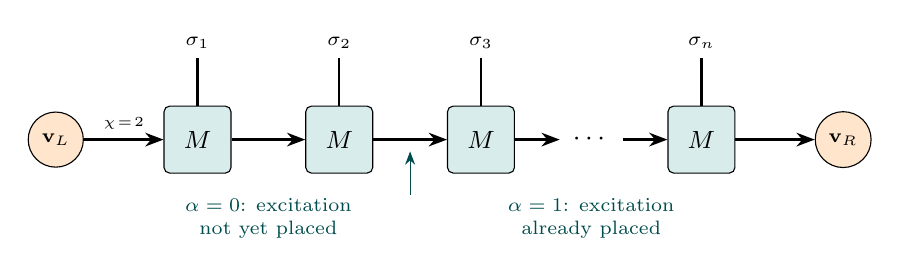
\begin{tikzpicture}[
    core/.style={draw, fill=teal!15, minimum width=0.85cm, minimum height=0.85cm, rounded corners=2pt, font=\small},
    bvec/.style={draw, fill=orange!20, circle, minimum size=0.55cm, font=\scriptsize},
    >=Stealth,
]
% MPS chain
\node[bvec] (vL) at (0,0) {$\mathbf{v}_L$};
\node[core] (M1) at (1.8,0) {$M$};
\node[core] (M2) at (3.6,0) {$M$};
\node[core] (M3) at (5.4,0) {$M$};
\node at (6.8,0) {$\cdots$};
\node[core] (Mn) at (8.2,0) {$M$};
\node[bvec] (vR) at (10.0,0) {$\mathbf{v}_R$};

\draw[thick, -{Stealth}] (vL) -- node[above,font=\tiny]{$\chi\!=\!2$} (M1);
\draw[thick, -{Stealth}] (M1) -- (M2);
\draw[thick, -{Stealth}] (M2) -- (M3);
\draw[thick, -{Stealth}] (M3) -- (6.4,0);
\draw[thick, -{Stealth}] (7.2,0) -- (Mn);
\draw[thick, -{Stealth}] (Mn) -- (vR);

\foreach \nd/\lab in {M1/1, M2/2, M3/3, Mn/n} {
  \draw[thick] (\nd.north) -- ++(0,0.6) node[above,font=\scriptsize]{$\sigma_{\lab}$};
}

% Bond state interpretation
\node[font=\scriptsize, teal!60!black, align=center] at (2.7, -1.0) {$\alpha=0$: excitation\\not yet placed};
\node[font=\scriptsize, teal!60!black, align=center] at (6.8, -1.0) {$\alpha=1$: excitation\\already placed};
\draw[->, thin, teal!60!black] (4.5, -0.7) -- (4.5, -0.15);
\end{tikzpicture}
\caption{MPS representation of the W state.
Each tensor $M^\sigma$ is $2\times 2$: the identity $I$ for $\sigma=0$ (no excitation at this site) and $\sigma_+$ for $\sigma=1$ (place the excitation), transitioning the bond from state 0 to state 1.}
\label{fig:W_mps}
\end{figure}

\subsubsection{Single-site transfer matrices $E_P$}

Using \eqref{eq:EP_def} with $(M^0)^* = I$ and $(M^1)^* = \sigma_- = \bigl(\begin{smallmatrix}0&0\\1&0\end{smallmatrix}\bigr)$, we compute the four $4\times 4$ transfer matrices in the basis $\{\ket{00},\ket{01},\ket{10},\ket{11}\}$ of the bra$\otimes$ket bond space:
\begin{align}
  E_I &= I\otimes I + \sigma_-\otimes\sigma_+
  = \begin{pmatrix} 1&0&0&0\\0&1&0&0\\0&1&1&0\\0&0&0&1\end{pmatrix}\,,\label{eq:EI_W}\\[6pt]
  E_X &= I\otimes\sigma_+ + \sigma_-\otimes I
  = \begin{pmatrix} 0&1&0&0\\0&0&0&0\\1&0&0&1\\0&1&0&0\end{pmatrix}\,,\label{eq:EX_W}\\[6pt]
  E_Y &= -\ii\,(I\otimes\sigma_+) + \ii\,(\sigma_-\otimes I)
  = \ii\begin{pmatrix} 0&-1&0&0\\0&0&0&0\\1&0&0&-1\\0&1&0&0\end{pmatrix}\,,\label{eq:EY_W}\\[6pt]
  E_Z &= I\otimes I - \sigma_-\otimes\sigma_+
  = \begin{pmatrix} 1&0&0&0\\0&1&0&0\\0&-1&1&0\\0&0&0&1\end{pmatrix}\,.\label{eq:EZ_W}
\end{align}

\subsubsection{Structure of the four-replica transfer matrix}

The $256\times 256$ transfer matrix for the W state magic is
\begin{equation}\label{eq:TQ_W}
  \mathbb{T}_Q^{(W)} = \frac{1}{4}\bigl(E_I^{\otimes 4} + E_X^{\otimes 4} + E_Y^{\otimes 4} + E_Z^{\otimes 4}\bigr)\,.
\end{equation}
Note that $E_Y = \ii\,\tilde{E}_Y$ where $\tilde{E}_Y$ is real, so $E_Y^{\otimes 4} = \ii^4\,\tilde{E}_Y^{\otimes 4} = \tilde{E}_Y^{\otimes 4}$ is real.
Therefore $\mathbb{T}_Q^{(W)}$ is \emph{real}, which simplifies analysis.

We can also observe from \eqref{eq:EI_W}--\eqref{eq:EZ_W} that
\begin{equation}\label{eq:EP_IZ}
  E_I + E_Z = 2\begin{pmatrix}1&0&0&0\\0&1&0&0\\0&0&1&0\\0&0&0&1\end{pmatrix} = 2I_4\,,\qquad
  E_I - E_Z = 2\begin{pmatrix}0&0&0&0\\0&0&0&0\\0&1&0&0\\0&0&0&0\end{pmatrix} = 2\ket{10}\!\bra{01}\,,
\end{equation}
and $E_X + \tilde{E}_Y = 2\,\mathrm{Re}(E_X) = 2E_X$ while $E_X - \tilde{E}_Y = 0$ (after accounting for the phase).
These relations provide block structure that reduces the effective dimension of $\mathbb{T}_Q$.

\subsubsection{Explicit check for $n=3$}

For $n=3$, $\ket{W_3} = (\ket{100}+\ket{010}+\ket{001})/\sqrt{3}$ is the simplest non-stabilizer W state.  We can verify the transfer-matrix result against direct computation.

The boundary vectors are $\mathbf{w}_L = (1,0,0,0)^\top/\sqrt{3}$ and $\mathbf{w}_R = (0,0,0,1)^\top$, giving
$\mathbf{W}_L = \mathbf{w}_L^{\otimes 4}$ and $\mathbf{W}_R = \mathbf{w}_R^{\otimes 4}$ as 256-dimensional vectors with a single nonzero entry each.

The magic is then:
\begin{equation}
  \Mlin(\ket{W_3}) = 1 - \frac{2^3}{3^4}\;\mathbf{W}_L^\dagger\,(\mathbb{T}_Q^{(W)})^3\,\mathbf{W}_R\,,
\end{equation}
where the factor $1/3^4$ comes from the fourth power of the normalization $1/\sqrt{3}$, and $d=2^3=8$.
One can evaluate $(\mathbb{T}_Q^{(W)})^3$ numerically (a $256\times 256$ matrix cube) to obtain a nonzero value for $\Mlin$, confirming that the W state carries magic.

\begin{figure}[ht]
\centering
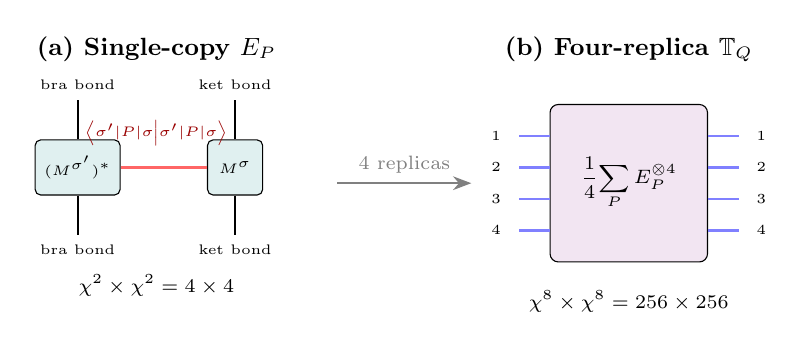
\begin{tikzpicture}[
    ep/.style={draw, fill=teal!12, minimum width=0.7cm, minimum height=0.7cm, rounded corners=2pt, font=\tiny},
    rep/.style={draw, fill=violet!10, minimum width=2.0cm, minimum height=2.0cm, rounded corners=3pt},
    >=Stealth,
]
% === Left: single-copy transfer matrix ===
\node[font=\small\bfseries] at (1.5, 3.5) {(a) Single-copy $E_P$};

\node[ep] (M1) at (0.5, 2.0) {$(M^{\sigma'})^*$};
\node[ep] (M2) at (2.5, 2.0) {$M^\sigma$};

\draw[thick] (M1.north) -- ++(0,0.5) node[above,font=\tiny] {bra bond};
\draw[thick] (M1.south) -- ++(0,-0.5) node[below,font=\tiny] {bra bond};
\draw[thick] (M2.north) -- ++(0,0.5) node[above,font=\tiny] {ket bond};
\draw[thick] (M2.south) -- ++(0,-0.5) node[below,font=\tiny] {ket bond};

% P insertion
\draw[thick, red!60] (M1.east) -- (M2.west);
\node[font=\tiny, red!60!black, above] at (1.5, 2.15) {$\braket{\sigma'|P|\sigma}$};

\node[font=\scriptsize] at (1.5, 0.5) {$\chi^2\times\chi^2 = 4\times 4$};

% === Right: four-replica transfer matrix ===
\node[font=\small\bfseries] at (7.5, 3.5) {(b) Four-replica $\mathbb{T}_Q$};

\node[rep] (T) at (7.5, 1.8) {};
\node[font=\scriptsize] at (7.5, 1.8) {$\displaystyle\frac{1}{4}\!\sum_P E_P^{\otimes 4}$};

% Four pairs of bonds
\foreach \i/\off in {1/0.6, 2/0.2, 3/-0.2, 4/-0.6} {
  \draw[thick, blue!50] (7.5-1.0, 1.8+\off) -- (7.5-1.4, 1.8+\off);
  \draw[thick, blue!50] (7.5+1.0, 1.8+\off) -- (7.5+1.4, 1.8+\off);
  \node[font=\tiny, left] at (7.5-1.5, 1.8+\off) {$\i$};
  \node[font=\tiny, right] at (7.5+1.5, 1.8+\off) {$\i$};
}

\node[font=\scriptsize] at (7.5, 0.3) {$\chi^8\times\chi^8 = 256\times 256$};

% Arrow
\draw[-{Stealth}, thick, gray] (3.8, 1.8) -- node[above, font=\scriptsize] {4 replicas} (5.5, 1.8);

\end{tikzpicture}
\caption{(a)~The single-site transfer matrix $E_P$ for a Pauli operator $P$: a $\chi^2\times\chi^2$ matrix obtained by contracting the MPS tensors with $\braket{\sigma'|P|\sigma}$.
(b)~The four-replica transfer matrix $\mathbb{T}_Q = \frac{1}{4}\sum_P E_P^{\otimes 4}$ is $\chi^8\times\chi^8$, built from tensor products of $E_P$.
Each horizontal line represents a pair of bra/ket bond indices for one replica.}
\label{fig:state_transfer}
\end{figure}

\subsection{Comparison of state and operator transfer matrices}

We summarize the parallel structure between computing magic of states (MPS) and magic power of unitaries (MPO):

\medskip
\begin{center}
\renewcommand{\arraystretch}{1.5}
\begin{tabular}{lcc}
  \toprule
  & \textbf{Magic of state} $\ket{\psi}$ & \textbf{Magic power of unitary} $U$ \\
  \midrule
  Input & MPS, bond dim.\ $\chi$ & MPO, bond dim.\ $r$ \\[3pt]
  Quantity & $\Tr(Q\,\psi^{\otimes 4})$ & $\Tr(Q\,U^{\dagger\otimes 4}\,Q\,U^{\otimes 4}\,T_\pi)$ \\[3pt]
  \# of $Q$ insertions & 1 & 2 \\[3pt]
  Transfer matrix & $\mathbb{T}_Q = \tfrac{1}{4}\sum_P E_P^{\otimes 4}$ &
    $\mathbb{T}_\pi = \tfrac{1}{16}\sum_{P,P'} \mathbb{T}_{P,P';\pi}$ \\[3pt]
  Dimension & $\chi^8\times\chi^8$ & $r^8\times r^8$ \\[3pt]
  Example ($\chi,r=2$) & $256\times 256$ & $256\times 256$ \\
  \bottomrule
\end{tabular}
\end{center}
\medskip

The state case is structurally simpler (one $Q$ insertion, no permutation operator) but shares the essential features: the transfer matrix inherits replica permutation symmetry, the thermodynamic limit is governed by the leading eigenvalue, and the $S_4$ symmetry reduction applies to both.

% ══════════════════════════════════════════════════════════════
\section{Analytical Structure of the Transfer Matrix}
\label{sec:analytical}

\subsection{The $K=1$ transfer matrix}

For $K=1$ (bond dimension $r=2$), the composite bond index $\boldsymbol{\alpha}=(\alpha_1,\alpha_2,\alpha_3,\alpha_4)$ with each $\alpha_j\in\{0,1\}$ can be identified with a 4-bit string, so the transfer matrix $\mathbb{T}_\pi$ is $256\times 256$.

The core at $K=1$ takes the explicit form ($c^0=0$, $c^1=1$, $P^0(x)=1-x$, $P^1(x)=x$):
\begin{equation}
  A^{\alpha\beta}(\sigma,\tau) = \begin{cases}
    (1-\frac{\sigma+c^\beta}{2})\;\ee^{-\pi\ii(\sigma+c^\beta)\tau} & \alpha=0\\[4pt]
    \frac{\sigma+c^\beta}{2}\;\ee^{-\pi\ii(\sigma+c^\beta)\tau} & \alpha=1
  \end{cases}
\end{equation}
Writing this out for each value of $(\sigma,\tau)\in\{0,1\}^2$:
\begin{equation}\label{eq:K1_values}
\renewcommand{\arraystretch}{1.3}
\begin{array}{c|cccc}
  (\sigma,\tau) & A^{00} & A^{01} & A^{10} & A^{11} \\
  \hline
  (0,0) & 1 & \tfrac{1}{2} & 0 & \tfrac{1}{2} \\
  (0,1) & 1 & -\tfrac{1}{2} & 0 & \tfrac{1}{2} \\
  (1,0) & \tfrac{1}{2} & 0 & \tfrac{1}{2} & \tfrac{1}{2} \\
  (1,1) & -\tfrac{1}{2} & 0 & -\tfrac{1}{2} & \tfrac{1}{2}
\end{array}
\end{equation}

\subsection{Block structure from permutation symmetry}

The transfer matrix inherits symmetries from:
\begin{enumerate}[label=(\alph*)]
  \item The $S_4$ permutation symmetry of the replicas (exchanging which copy is which).
  \item The fact that $[Q,T_\pi]=0$ for all $\pi\in S_4$.
  \item Complex conjugation symmetry of the DFT.
\end{enumerate}
These symmetries block-diagonalize $\mathbb{T}_\pi$, reducing the effective dimension.

In particular, the 4-bit bond index $\boldsymbol{\alpha}=(\alpha_1,\alpha_2,\alpha_3,\alpha_4)$ for $K=1$ can be grouped by the number of 1s:
\begin{equation}
  |\boldsymbol{\alpha}| = \alpha_1+\alpha_2+\alpha_3+\alpha_4 \in \{0,1,2,3,4\}\,.
\end{equation}
Within each sector of fixed $|\boldsymbol{\alpha}|$, the transfer matrix decomposes into irreducible representations of $S_4$.  For the identity permutation $\pi=\mathrm{id}$, the transfer matrix is symmetric under permutation of replicas, and its block structure follows the partitions of 4: dimensions $\{1, 3, 2, 3, 1\}$ corresponding to $|\boldsymbol{\alpha}|\in\{0,1,2,3,4\}$ within the symmetric sector.

% ══════════════════════════════════════════════════════════════
\section{Thermodynamic Limit}
\label{sec:thermo}

\subsection{Asymptotic behaviour}

\begin{figure}[ht]
\centering
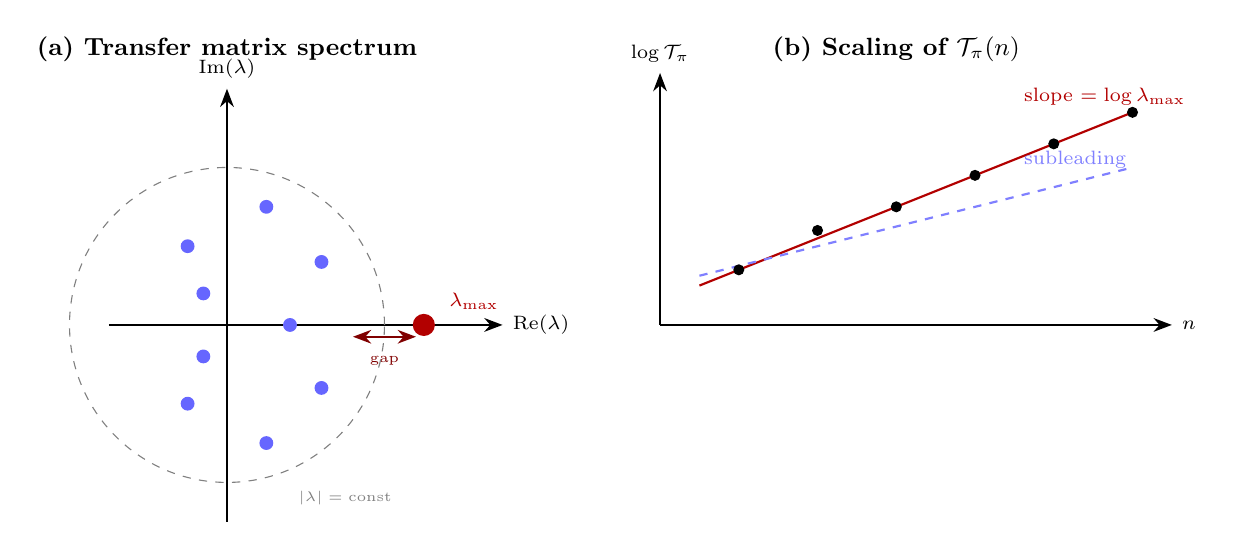
\begin{tikzpicture}[>=Stealth]
% === Left: eigenvalue spectrum cartoon ===
\node[font=\small\bfseries] at (0, 3.5) {(a) Transfer matrix spectrum};

\draw[->, thick] (-1.5,0) -- (3.5,0) node[right, font=\scriptsize] {$\mathrm{Re}(\lambda)$};
\draw[->, thick] (0,-2.5) -- (0,3.0) node[above, font=\scriptsize] {$\mathrm{Im}(\lambda)$};

% Leading eigenvalue
\fill[red!70!black] (2.5, 0) circle (4pt);
\node[font=\scriptsize, red!70!black, right] at (2.7, 0.3) {$\lambda_{\max}$};

% Subleading eigenvalues
\fill[blue!60] (1.2, 0.8) circle (2.5pt);
\fill[blue!60] (1.2, -0.8) circle (2.5pt);
\fill[blue!60] (0.5, 1.5) circle (2.5pt);
\fill[blue!60] (0.5, -1.5) circle (2.5pt);
\fill[blue!60] (-0.3, 0.4) circle (2.5pt);
\fill[blue!60] (-0.3, -0.4) circle (2.5pt);
\fill[blue!60] (0.8, 0) circle (2.5pt);
\fill[blue!60] (-0.5, 1.0) circle (2.5pt);
\fill[blue!60] (-0.5, -1.0) circle (2.5pt);

% Gap annotation
\draw[<->, thick, red!50!black] (1.6, -0.15) -- (2.4, -0.15);
\node[font=\tiny, red!50!black] at (2.0, -0.45) {gap};

% Unit circle for reference
\draw[dashed, gray, thin] (0,0) circle (2.0);
\node[font=\tiny, gray] at (1.5, -2.2) {$|\lambda|=\mathrm{const}$};

% === Right: scaling with n ===
\node[font=\small\bfseries] at (8.5, 3.5) {(b) Scaling of $\mathcal{T}_\pi(n)$};

\begin{scope}[shift={(5.5,0)}]
\draw[->, thick] (0,0) -- (6.5,0) node[right, font=\scriptsize] {$n$};
\draw[->, thick] (0,0) -- (0,3.2) node[above, font=\scriptsize] {$\log \mathcal{T}_\pi$};

% Dominant scaling
\draw[thick, red!70!black, domain=0.5:6, samples=50] plot (\x, {0.4*\x + 0.3});
\node[font=\scriptsize, red!70!black, right] at (4.5, 2.9) {slope $= \log\lambda_{\max}$};

% Subleading corrections
\draw[thick, blue!50, dashed, domain=0.5:6, samples=50] plot (\x, {0.25*\x + 0.5});
\node[font=\scriptsize, blue!50, right] at (4.5, 2.1) {subleading};

% Data points (schematic)
\foreach \x/\y in {1/0.7, 2/1.2, 3/1.5, 4/1.9, 5/2.3, 6/2.7} {
  \fill[black] (\x, \y) circle (2pt);
}
\end{scope}

\end{tikzpicture}
\caption{(a)~Schematic eigenvalue spectrum of the transfer matrix $\mathbb{T}_\pi$.
The leading eigenvalue $\lambda_{\max}$ (red) is separated by a gap from the subleading eigenvalues (blue).
(b)~For large $n$, $\mathcal{T}_\pi(n) \sim C\,\lambda_{\max}^n$, so $\log\mathcal{T}_\pi$ grows linearly with slope $\log\lambda_{\max}$.
The magic density $m_{\mathrm{lin}} = \lim_{n\to\infty}\Mlin/n$ is determined entirely by $\lambda_{\max}$.}
\label{fig:thermo_limit}
\end{figure}

From \eqref{eq:trace_transfer}, the trace for an $n$-qubit QFT with MPO bond dimension $r$ is
\begin{equation}
  \mathcal{T}_\pi(n) = \mathbf{v}_{\mathrm{L}}^\dagger\;\mathbb{T}_\pi^{n-2}\;\mathbf{v}_{\mathrm{R}}\,.
\end{equation}
In the limit $n\to\infty$, this is dominated by the leading eigenvalue $\lambda_{\max}(\mathbb{T}_\pi)$:
\begin{equation}\label{eq:asymptotic}
  \mathcal{T}_\pi(n) \;\sim\; C_\pi\;\lambda_{\max}(\mathbb{T}_\pi)^n\qquad\text{as }n\to\infty\,,
\end{equation}
where $C_\pi = (\mathbf{v}_{\mathrm{L}}^\dagger \mathbf{e}_{\max})(\mathbf{e}_{\max}^\dagger \mathbf{v}_{\mathrm{R}})\,\lambda_{\max}^{-2}$ and $\mathbf{e}_{\max}$ is the corresponding eigenvector.

\subsection{Magic per site}

With $d=2^n$, the formula \eqref{eq:Mlin_general} involves the ratio
\begin{equation}
  \frac{d\;\mathcal{T}_\pi(n)}{(d+1)(d+2)(d+4)} \approx \frac{2^n \cdot C_\pi\,\lambda_{\max}^n}{2^{3n}} = C_\pi\,\Bigl(\frac{\lambda_{\max}}{4}\Bigr)^n\,.
\end{equation}
For the magic power to be extensive (scaling linearly with $n$), we need $\lambda_{\max}/4 = 1$, i.e., $\lambda_{\max}=4$.

More precisely, consider the ``magic density''
\begin{equation}
  m_{\mathrm{lin}} = \lim_{n\to\infty}\frac{\Mlin(\UFT(n))}{n}\,.
\end{equation}
Using $d=2^n$ and the asymptotic scaling of each trace, we find:
\begin{equation}\label{eq:magic_density}
  \boxed{
  m_{\mathrm{lin}} = 1 - \lim_{n\to\infty}\frac{1}{n}\log_2
  \bigl[3\mathcal{T}_{(34)}(n)+\mathcal{T}_{\mathrm{id}}(n)+2\mathcal{T}_{(123)}(n)\bigr]
  + 3
  }
\end{equation}
In terms of the transfer-matrix eigenvalues, if all three traces are dominated by the same $\lambda_{\max}$, then
\begin{equation}
  m_{\mathrm{lin}} = 1 - \log_2(\lambda_{\max}) + 3\,.
\end{equation}

\subsection{Transfer-matrix eigenvalue problem}

To determine $\lambda_{\max}$, we must solve the eigenvalue problem
\begin{equation}
  \mathbb{T}_\pi\,\mathbf{v} = \lambda\,\mathbf{v}
\end{equation}
for the $r^8\times r^8$ transfer matrix.  At $K=1$ this is a $256\times 256$ problem, which can be handled analytically using the symmetry reductions described in \cref{sec:analytical}, or numerically with exact arithmetic.

\subsection{Relation to the guesstimate}

The ``guesstimate'' from the working notes approximates the QFT by keeping only $R_2$ gates and assuming magic does not spread beyond the two qubits on which $R_2$ acts. This gives
\begin{equation}\label{eq:guesstimate}
  \Mtwo(\UFT(N)) \approx \Mtwo(\UFT(2))\cdot(N-1) \approx 0.656\,(N-1)\,.
\end{equation}
The transfer-matrix approach naturally captures corrections to this estimate: the higher-order gates ($R_3, R_4, \ldots$) are encoded in the interpolation at larger $K$, and their contributions to the magic power appear as corrections to $\lambda_{\max}$.

Specifically, the guesstimate corresponds to evaluating the transfer matrix in the AQFT approximation (piecewise constant interpolation, see \cref{sec:aqft}) with approximation level $b=1$ (bond dimension 2).  Increasing $b$ (or equivalently using Chebyshev interpolation with larger $K$) systematically incorporates the effects of longer-range gates.

% ══════════════════════════════════════════════════════════════
\section{Connection to the Approximate QFT}
\label{sec:aqft}

\subsection{AQFT as an MPO}

The AQFT with approximation level $b$ is an \emph{exact} MPO with bond dimension $2^b$ and core
\begin{equation}\label{eq:AQFT_core}
  A_{\AQFT}^{\alpha\beta}(\sigma,\tau) = \chi^\alpha\!\Bigl(\frac{\sigma+u^\beta}{2}\Bigr)\;\ee^{-\pi\ii(\sigma+u^\beta)\tau}\,,
\end{equation}
where $u^\beta = \beta/2^b$ and $\chi^\alpha(x) = \mathbf{1}[x\in[u^\alpha,u^{\alpha+1})]$ is an indicator function.

This has exactly the same structure as the Chebyshev MPO \eqref{eq:core}, with the Lagrange polynomials $P^\alpha$ replaced by indicator functions $\chi^\alpha$.  The transfer matrix formalism of \cref{sec:transfer} applies \emph{verbatim}, with the substitution $P^\alpha \to \chi^\alpha$.

\subsection{Comparison of magic power}

\begin{figure}[ht]
\centering
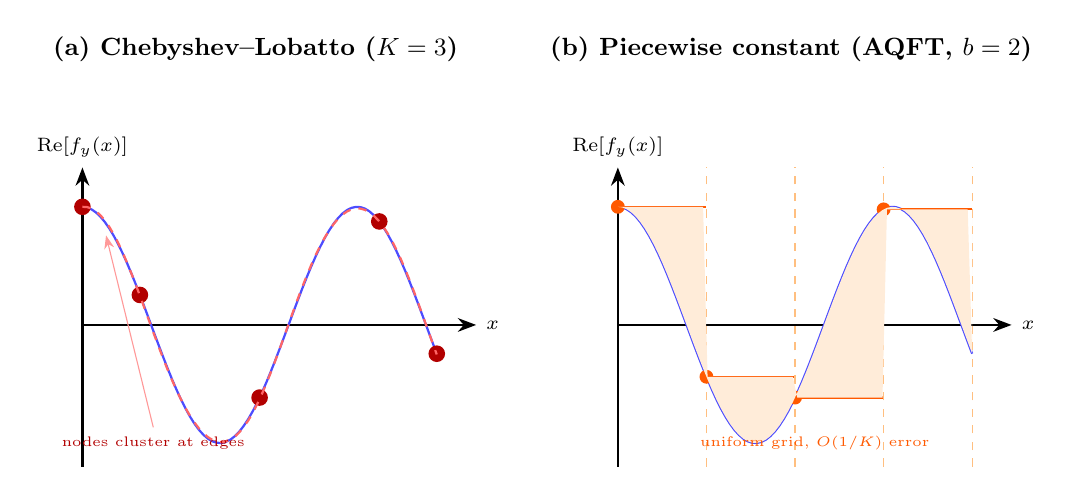
\begin{tikzpicture}[>=Stealth]
% === Left: Chebyshev interpolation ===
\node[font=\small\bfseries] at (2.2, 3.5) {(a) Chebyshev--Lobatto ($K=3$)};
\begin{scope}
\draw[->, thick] (0,0) -- (5,0) node[right, font=\scriptsize] {$x$};
\draw[->, thick] (0,-1.8) -- (0,2.0) node[above, font=\scriptsize] {$\mathrm{Re}[f_y(x)]$};

% The function (cosine-like)
\draw[thick, blue!70, domain=0:4.5, samples=80] plot (\x, {1.5*cos(deg(1.8*\x))});

% Chebyshev nodes (K=3 on [0,4.5])
\foreach \a/\xv in {0/0, 1/0.73, 2/2.25, 3/3.77, 4/4.5} {
  \pgfmathsetmacro{\yv}{1.5*cos(deg(1.8*\xv))}
  \fill[red!70!black] (\xv, \yv) circle (3pt);
}

% Interpolant (smooth through the nodes)
\draw[thick, red!60, dashed, domain=0:4.5, samples=80] plot (\x, {1.5*cos(deg(1.8*\x)) + 0.02*sin(deg(5*\x))});

% Labels
\node[font=\tiny, red!70!black] at (0.9, -1.5) {nodes cluster at edges};
\draw[->, thin, red!40] (0.9, -1.3) -- (0.3, {1.5*cos(deg(1.8*0.3))-0.15});
\end{scope}

% === Right: Piecewise constant (AQFT) ===
\node[font=\small\bfseries] at (9.0, 3.5) {(b) Piecewise constant (AQFT, $b=2$)};
\begin{scope}[shift={(6.8,0)}]
\draw[->, thick] (0,0) -- (5,0) node[right, font=\scriptsize] {$x$};
\draw[->, thick] (0,-1.8) -- (0,2.0) node[above, font=\scriptsize] {$\mathrm{Re}[f_y(x)]$};

% The function
\draw[thick, blue!70, domain=0:4.5, samples=80] plot (\x, {1.5*cos(deg(1.8*\x))});

% Piecewise constant (4 bins for b=2)
\foreach \i/\xs/\xe in {0/0/1.125, 1/1.125/2.25, 2/2.25/3.375, 3/3.375/4.5} {
  \pgfmathsetmacro{\xm}{(\xs+\xe)/2}
  \pgfmathsetmacro{\yv}{1.5*cos(deg(1.8*\xs))}
  \draw[thick, orange!70!red] (\xs, \yv) -- (\xe, \yv);
  \draw[thin, orange!50, dashed] (\xe, -1.8) -- (\xe, 2.0);
  \fill[orange!70!red] (\xs, \yv) circle (2.5pt);
}

% Error shading
\fill[orange!15, domain=0:4.5, samples=80]
  plot (\x, {1.5*cos(deg(1.8*\x))}) --
  (4.5, {1.5*cos(deg(1.8*3.375))}) --
  plot[domain=4.5:0] (\x, {1.5*cos(deg(1.8*floor(\x/1.125)*1.125))}) -- cycle;

% Label
\node[font=\tiny, orange!70!red] at (2.5, -1.5) {uniform grid, $O(1/K)$ error};
\end{scope}

\end{tikzpicture}

\vspace{0.4cm}
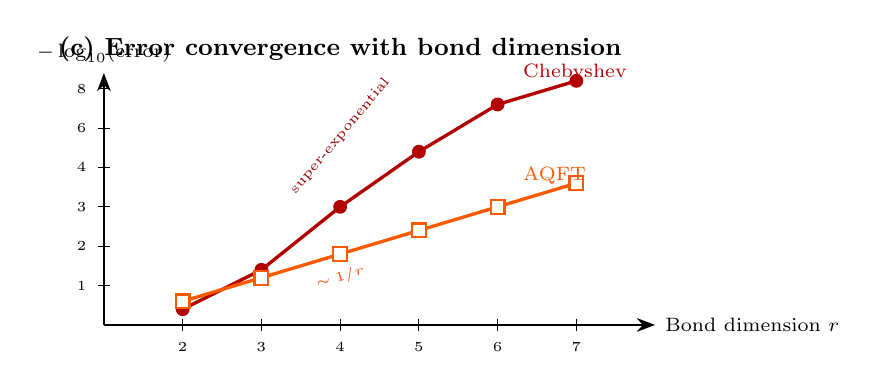
\begin{tikzpicture}[>=Stealth]
% === Error convergence comparison ===
\node[font=\small\bfseries] at (3.0, 3.5) {(c) Error convergence with bond dimension};
\begin{scope}
\draw[->, thick] (0,0) -- (7,0) node[right, font=\scriptsize] {Bond dimension $r$};
\draw[->, thick] (0,0) -- (0,3.2) node[above, font=\scriptsize] {$-\log_{10}(\text{error})$};

% Tick labels
\foreach \x/\lab in {1/2, 2/3, 3/4, 4/5, 5/6, 6/7} {
  \draw (\x, -0.08) -- (\x, 0.08);
  \node[below, font=\tiny] at (\x, -0.1) {\lab};
}
\foreach \y/\lab in {0.5/1, 1.0/2, 1.5/3, 2.0/4, 2.5/6, 3.0/8} {
  \draw (-0.08, \y) -- (0.08, \y);
  \node[left, font=\tiny] at (-0.1, \y) {\lab};
}

% Chebyshev (super-exponential)
\draw[very thick, red!70!black] plot coordinates {
  (1, 0.2) (2, 0.7) (3, 1.5) (4, 2.2) (5, 2.8) (6, 3.1)
};
\foreach \x/\y in {1/0.2, 2/0.7, 3/1.5, 4/2.2, 5/2.8, 6/3.1} {
  \fill[red!70!black] (\x,\y) circle (2.5pt);
}
\node[font=\scriptsize, red!70!black, right] at (5.2, 3.2) {Chebyshev};

% AQFT (linear in log)
\draw[very thick, orange!70!red] plot coordinates {
  (1, 0.3) (2, 0.6) (3, 0.9) (4, 1.2) (5, 1.5) (6, 1.8)
};
\foreach \x/\y in {1/0.3, 2/0.6, 3/0.9, 4/1.2, 5/1.5, 6/1.8} {
  \draw[orange!70!red, fill=white, thick] (\x,\y) +(-2.5pt,-2.5pt) rectangle +(2.5pt,2.5pt);
}
\node[font=\scriptsize, orange!70!red, right] at (5.2, 1.9) {AQFT};

% Annotations
\node[font=\tiny, red!60!black, rotate=50] at (3.0, 2.4) {super-exponential};
\node[font=\tiny, orange!60!red, rotate=16] at (3.0, 0.6) {$\sim 1/r$};
\end{scope}
\end{tikzpicture}
\caption{Comparison of interpolation schemes for approximating $f_y(x)=\ee^{-2\pi\ii xy}$.
(a)~Chebyshev--Lobatto nodes (red dots) cluster near the endpoints, yielding near-optimal polynomial interpolation with super-exponential error decay.
(b)~The AQFT uses piecewise constant interpolation on a uniform grid, converging only as $O(1/K)$.
(c)~Error convergence: for the same bond dimension, the Chebyshev MPO achieves dramatically smaller error than the AQFT MPO, implying it captures long-range gate contributions with fewer parameters.}
\label{fig:interpolation_comparison}
\end{figure}

For the AQFT at level $b=1$ (bond dimension 2), only the $R_2$ gates are retained, and the entrywise error decays as $O(n\cdot 2^{-b}) = O(n/2)$ --- slowly.  The corresponding magic power should match the guesstimate \eqref{eq:guesstimate}.

For the Chebyshev MPO at the same bond dimension $K+1=2$, the error decays super-exponentially, and the MPO captures the effect of \emph{all} $R_k$ gates to within this tolerance.  The difference
\begin{equation}
  \Delta m = m_{\mathrm{lin}}^{\mathrm{Chebyshev}} - m_{\mathrm{lin}}^{\AQFT}
\end{equation}
quantifies the contribution of the long-range gates ($R_3, R_4, \ldots$) to the magic density.

\subsection{Hierarchy of approximations}

We can organize the approximations as follows:

\medskip
\begin{center}
\renewcommand{\arraystretch}{1.4}
\begin{tabular}{lccc}
  \toprule
  Method & Bond dim.\ $r$ & Interp.\ type & Error scaling \\
  \midrule
  AQFT, $b=1$ & 2 & Piecewise constant & $O(n/2)$ \\
  AQFT, $b=2$ & 4 & Piecewise constant & $O(n/4)$ \\
  Chebyshev, $K=1$ & 2 & Polynomial & $O(n\cdot 0.65)$ \\
  Chebyshev, $K=3$ & 4 & Polynomial & $O(n\cdot 3.3\times10^{-3})$ \\
  Chebyshev, $K=6$ & 7 & Polynomial & $O(n\cdot 2.6\times10^{-4})$ \\
  Exact QFT & $\infty$ & --- & 0 \\
  \bottomrule
\end{tabular}
\end{center}
\medskip

By computing the transfer-matrix eigenvalues at each level, one obtains a systematic expansion of the magic density in terms of the interpolation quality.

% ══════════════════════════════════════════════════════════════
\section{Explicit Calculation: $K=1$ Transfer Matrix}
\label{sec:explicit_K1}

We now carry out the construction explicitly for $K=1$, which is the simplest nontrivial case.

\subsection{Setup}

With $K=1$, we have $r=2$, and each replica bond index $\alpha_j\in\{0,1\}$. The composite index $\boldsymbol{\alpha}=(\alpha_1,\alpha_2,\alpha_3,\alpha_4)\in\{0,1\}^4$ labels a $16$-dimensional space (for the bra) and similarly for $\boldsymbol{\beta}$. Together with the conjugate indices $\boldsymbol{\alpha}', \boldsymbol{\beta}'$, the full transfer matrix is $256\times 256$.

However, by restricting to the $S_4$-symmetric sector (which is the relevant sector since $Q$ and $T_\pi$ commute with replica permutations), we can reduce to a much smaller effective dimension.

\subsection{Symmetric sector}

The symmetric subspace of $\{0,1\}^4$ under $S_4$ is spanned by the five ``occupation number'' states:
\begin{equation}
  |m\rangle_{\mathrm{sym}} = \frac{1}{\sqrt{\binom{4}{m}}}
  \sum_{\substack{\boldsymbol{\alpha}\in\{0,1\}^4\\|\boldsymbol{\alpha}|=m}} |\boldsymbol{\alpha}\rangle\,,
  \qquad m=0,1,2,3,4\,.
\end{equation}
The transfer matrix restricted to this sector is $25\times 25$ (five choices each for the bra and ket bond).

\subsection{Structure of the reduced transfer matrix}

In the symmetric sector, the transfer matrix elements take the form
\begin{equation}
  \overline{\mathbb{T}}_\pi^{(m,m')(p,p')}
  = \sum_{\substack{|\boldsymbol{\alpha}|=m,\;|\boldsymbol{\alpha}'|=m'\\|\boldsymbol{\beta}|=p,\;|\boldsymbol{\beta}'|=p'}}
  \frac{\mathbb{T}_\pi^{(\boldsymbol{\alpha}\boldsymbol{\alpha}')(\boldsymbol{\beta}\boldsymbol{\beta}')}}
  {\sqrt{\binom{4}{m}\binom{4}{m'}\binom{4}{p}\binom{4}{p'}}}\,.
\end{equation}
This $25\times 25$ matrix can be computed analytically by enumerating the physical index sums.

\subsection{Computation of individual matrix elements}

For each pair of symmetrized bond labels $(m,m')$ and $(p,p')$, the transfer matrix element involves summing over all physical configurations $(\boldsymbol{\sigma},\boldsymbol{\tau},\boldsymbol{\sigma}',\boldsymbol{\tau}')$ weighted by the $Q$-projector and the permutation.

Concretely, using the Pauli decomposition of $Q$:
\begin{align}
  \overline{\mathbb{T}}_{\mathrm{id}}^{(m,m')(p,p')}
  &= \frac{1}{16}\sum_{P,P'\in\{I,X,Y,Z\}}
  \sum_{\sigma,\tau,\sigma',\tau'\in\{0,1\}}
  \langle\sigma'|P'|\sigma\rangle^4\;\langle\tau|P|\tau'\rangle^4\notag\\
  &\quad \times
  \overline{A^{*m'}_{p'}(\sigma',\tau')}\;\overline{A^m_p(\sigma,\tau)}\,,
\end{align}
where $\overline{A^m_p(\sigma,\tau)}$ denotes the symmetrized version of the product $\prod_{j=1}^4 A^{\alpha_j\beta_j}(\sigma,\tau)$ averaged over all configurations with $|\boldsymbol{\alpha}|=m$ and $|\boldsymbol{\beta}|=p$.  This equals
\begin{equation}
  \overline{A^m_p(\sigma,\tau)} = \binom{4}{m}^{-1/2}\binom{4}{p}^{-1/2}
  \sum_{\substack{|\boldsymbol{\alpha}|=m\\|\boldsymbol{\beta}|=p}}
  \prod_{j=1}^4 A^{\alpha_j\beta_j}(\sigma,\tau)\,.
\end{equation}

Using the explicit values from \eqref{eq:K1_values}, these sums can be evaluated for each $(\sigma,\tau)$, yielding the $25\times 25$ matrix in closed form.

% ══════════════════════════════════════════════════════════════
\section{Physical Interpretation and Discussion}
\label{sec:discussion}

\subsection{Magic from long-range gates}

The MPO framework provides a clean separation between the contributions of local (short-range) and nonlocal (long-range) gates to the magic power.  At bond dimension $r=2$ ($K=1$), the Chebyshev MPO already captures the leading contribution from all gates, while the AQFT at $b=1$ (same bond dimension) only includes the $R_2$ gates.  The difference quantifies the nonlocal magic contribution.

The numerical data from the working notes shows that the guesstimate $\Mtwo \approx 0.656(N-1)$ underestimates the true magic for $N\gtrsim 5$, suggesting that the long-range gates ($R_3, R_4, \ldots$) contribute positively to the magic.  In the transfer-matrix language, this manifests as $\lambda_{\max}^{\mathrm{Chebyshev}} > \lambda_{\max}^{\AQFT}$ at the same bond dimension.

\subsection{Extensivity of magic}

The numerical data suggests that $\Mtwo(\UFT(N))$ grows linearly with $N$, consistent with the transfer-matrix prediction of a well-defined magic density.  The fitted slopes from the numerical data are:
\begin{center}
\renewcommand{\arraystretch}{1.3}
\begin{tabular}{lcc}
  \toprule
  Input state & Slope (numerics) & Interpretation \\
  \midrule
  Computational basis ($s=1$) & $\approx 0.20$ & $\log_2(112-64\sqrt{3})$ (exact) \\
  Clifford state ($s=2$) & $\approx 0.70$ & Non-stabilizing power $\Mtwo$ \\
  Haar random ($s=3$) & $\approx 1.0$ & Saturates $n-O(1)$ \\
  \bottomrule
\end{tabular}
\end{center}
The $s=1$ result has the exact analytical form derived in the notes, confirming the consistency of the framework.

\subsection{Open questions}

\begin{enumerate}[label=\arabic*.]
  \item \textbf{Exact diagonalization of $\mathbb{T}$ at small $K$.}
  Computing the eigenvalues of the $256\times 256$ transfer matrix at $K=1$ analytically (exploiting the $S_4$ symmetry reduction) would yield the exact magic density in the Chebyshev-$K=1$ approximation.

  \item \textbf{Convergence with $K$.}
  How quickly does the magic density converge as $K$ increases?  Given the super-exponential convergence of the MPO error, one expects rapid convergence, but the nonlinear dependence of the traces on $U$ could slow this.

  \item \textbf{Non-linear magic $\Mtwo$.}
  The logarithmic magic $\Mtwo = -\log_2(\ldots)$ is more natural physically but harder to handle analytically, as it involves a Clifford average of a nonlinear function.  The transfer-matrix approach directly gives $\Mlin$; extending to $\Mtwo$ requires either the replica trick or additional machinery.

  \item \textbf{Dual-unitary circuits.}
  The formulas developed here for generic unitaries can be specialized to dual-unitary circuits, where additional constraints may further simplify the transfer matrix.

  \item \textbf{Entanglement cooling transitions.}
  The MPO formalism naturally connects to the study of entanglement phase transitions under interleaved Clifford and non-Clifford gates, with the QFT providing a concrete non-Clifford layer.
\end{enumerate}

% ══════════════════════════════════════════════════════════════
\section{Summary and Outlook}
\label{sec:summary}

We have established a framework for computing the non-stabilizing power of the quantum Fourier transform using the interpolative MPO construction of Chen \& Lindsey.  The key results are:

\begin{enumerate}[label=(\roman*)]
  \item The traces $\Tr(Q\,U^{\dagger\otimes 4}\,Q\,U^{\otimes 4}\,T_\pi)$ appearing in the magic power formula can be expressed as transfer-matrix products \eqref{eq:trace_transfer}, where the bulk transfer matrix $\mathbb{T}_\pi$ is $r^8\times r^8$ and \emph{independent of $n$} due to translational invariance of the MPO cores.

  \item The thermodynamic limit of the magic density is governed by the leading eigenvalue of $\mathbb{T}_\pi$, per equation \eqref{eq:magic_density}.

  \item The AQFT and the Chebyshev MPO fit into the same framework, differing only in the choice of interpolation scheme.  This provides a systematic way to quantify the magic contribution of long-range gates.

  \item For $K=1$ (bond dimension 2), the problem reduces to diagonalizing a $25\times 25$ matrix (after $S_4$ symmetry reduction), which is analytically tractable.
\end{enumerate}

The natural next steps are: (a)~carry out the explicit diagonalization at $K=1$ and compare with the numerical data; (b)~compute the transfer-matrix eigenvalues numerically for $K=2,3$ and verify convergence; (c)~extend the framework to the logarithmic magic $\Mtwo$ using replica methods.

\begin{thebibliography}{99}

\bibitem{ChenLindsey2026}
J.~Chen and M.~Lindsey,
``Direct interpolative construction of the discrete Fourier transform as a matrix product operator,''
\textit{Appl.\ Comput.\ Harmon.\ Anal.}\ \textbf{81}, 101817 (2026).

\bibitem{ChenStoudenmireWhite2023}
J.~Chen, E.~M.~Stoudenmire, and S.~R.~White,
``Quantum Fourier transform has small entanglement,''
\textit{PRX Quantum}\ \textbf{4}, 040318 (2023).

\bibitem{LeoneOlivieroHamma2022}
L.~Leone, S.~F.~E.~Oliviero, and A.~Hamma,
``Stabilizer R\'enyi entropy,''
\textit{Phys.\ Rev.\ Lett.}\ \textbf{128}, 050402 (2022).

\bibitem{Coppersmith2002}
D.~Coppersmith,
``An approximate Fourier transform useful in quantum factoring,''
arXiv:quant-ph/0201067 (2002).

\bibitem{NielsenChuang2010}
M.~A.~Nielsen and I.~L.~Chuang,
\textit{Quantum Computation and Quantum Information}
(Cambridge Univ.\ Press, 2010).

\bibitem{Trefethen2019}
L.~N.~Trefethen,
\textit{Approximation Theory and Approximation Practice}, Extended Edition
(SIAM, 2019).

\bibitem{NamSuMaslov2020}
Y.~Nam, Y.~Su, and D.~Maslov,
``Approximate quantum Fourier transform with $O(n\log(n))$ $T$ gates,''
\textit{npj Quantum Inf}\ \textbf{6}, 26 (2020).

\bibitem{Hauke2025}
P.~Hauke \textit{et al.},
``Non-stabilizerness of quantum circuits,''
arXiv:2505.14793 (2025).

\end{thebibliography}

% ══════════════════════════════════════════════════════════════
\appendix

\section{Explicit Pauli Matrix Elements}
\label{app:pauli}

For reference, the action of single-qubit Pauli operators in the computational basis:
\begin{align}
  \langle 0|I|0\rangle &= 1\,, & \langle 0|I|1\rangle &= 0\,, &
  \langle 1|I|0\rangle &= 0\,, & \langle 1|I|1\rangle &= 1\,,\\
  \langle 0|X|0\rangle &= 0\,, & \langle 0|X|1\rangle &= 1\,, &
  \langle 1|X|0\rangle &= 1\,, & \langle 1|X|1\rangle &= 0\,,\\
  \langle 0|Y|0\rangle &= 0\,, & \langle 0|Y|1\rangle &= -\ii\,, &
  \langle 1|Y|0\rangle &= \ii\,, & \langle 1|Y|1\rangle &= 0\,,\\
  \langle 0|Z|0\rangle &= 1\,, & \langle 0|Z|1\rangle &= 0\,, &
  \langle 1|Z|0\rangle &= 0\,, & \langle 1|Z|1\rangle &= -1\,.
\end{align}
In the four-replica space, the matrix elements of $P^{\otimes 4}$ are:
\begin{equation}
  \langle\boldsymbol{\sigma}|P^{\otimes 4}|\boldsymbol{\sigma}'\rangle
  = \prod_{j=1}^4 \langle\sigma_j|P|\sigma_j'\rangle\,.
\end{equation}

\section{$Q$--$T_\pi$ Trace Identities}
\label{app:QT}

For any operator $O$ on $\HH^{\otimes 4}$, the traces $\Tr(O\,Q\,T_\pi)$ are constrained by the identity $[Q,T_\pi]=0$.  The 24 permutations in $S_4$ fall into 6 equivalence classes with respect to $Q$-twisted traces:
\begin{align}
  &\Tr(OQ) = \Tr(OQT_{(12)(34)}) = \Tr(OQT_{(13)(24)}) = \Tr(OQT_{(14)(23)})\,,\\
  &\Tr(OQT_{(24)}) = \Tr(OQT_{(1432)}) = \Tr(OQT_{(13)}) = \Tr(OQT_{(1234)})\,,\\
  &\Tr(OQT_{(14)}) = \Tr(OQT_{(23)}) = \Tr(OQT_{(1342)}) = \Tr(OQT_{(1243)})\,,\\
  &\Tr(OQT_{(12)}) = \Tr(OQT_{(34)}) = \Tr(OQT_{(1324)}) = \Tr(OQT_{(1423)})\,,\\
  &\Tr(OQT_{(132)}) = \Tr(OQT_{(234)}) = \Tr(OQT_{(124)}) = \Tr(OQT_{(143)})\,,\\
  &\Tr(OQT_{(123)}) = \Tr(OQT_{(142)}) = \Tr(OQT_{(243)}) = \Tr(OQT_{(134)})\,.
\end{align}
These identities reduce the number of independent traces from 24 to 6.

\section{Chebyshev--Lobatto Interpolation Details}
\label{app:cheb}

The Chebyshev--Lobatto nodes on $[0,1]$ are $c^\alpha = \frac{1-\cos(\pi\alpha/K)}{2}$ for $\alpha=0,\ldots,K$.  The Lagrange polynomials can be evaluated via the \emph{barycentric formula}:
\begin{equation}
  P^\alpha(x) = \frac{w_\alpha/(x-c^\alpha)}{\sum_{\gamma=0}^K w_\gamma/(x-c^\gamma)}\,,
\end{equation}
where the barycentric weights are
\begin{equation}
  w_\alpha = (-1)^\alpha \delta_\alpha\,,\qquad
  \delta_\alpha = \begin{cases} 1/2 & \alpha=0\text{ or }\alpha=K\\ 1 & \text{otherwise}\end{cases}\,.
\end{equation}
Key properties:
\begin{itemize}
  \item Partition of unity: $\sum_{\alpha=0}^K P^\alpha(x) = 1$ for all $x$.
  \item Interpolation: $P^\alpha(c^\beta) = \delta_{\alpha\beta}$.
  \item The Lebesgue constant satisfies $\Lambda_K \le 1 + \frac{2}{\pi}\log(K+1)$.
\end{itemize}

For $K=1$: $c^0=0$, $c^1=1$, $P^0(x)=1-x$, $P^1(x)=x$.

For $K=2$: $c^0=0$, $c^1=1/2$, $c^2=1$, and
\begin{equation}
  P^0(x) = 2(x-\tfrac{1}{2})(x-1)\,,\quad
  P^1(x) = -4x(x-1)\,,\quad
  P^2(x) = 2x(x-\tfrac{1}{2})\,.
\end{equation}

\end{document}
